\documentclass{article}
%Usepackages
\usepackage{adjustbox, amsmath, amssymb, amsthm, blindtext, bm, bbm, dblfloatfix, esint, fancyhdr, float, graphicx, letltxmacro, marginnote, mathtools, subcaption, xcolor, titlesec, esint}
\usepackage{amssymb}
\usepackage[font={small, it}]{caption}
\usepackage{amsmath}
\usepackage{floatrow}
\usepackage{times}
\usepackage{ stmaryrd }
\usepackage{amsthm}
\usepackage{xcolor}
\usepackage{mathrsfs}
\usepackage[colorlinks = true,
            linkcolor = black,
            urlcolor  = blue,
            citecolor = black,
            anchorcolor = blue]{hyperref}
% \usepackage[mathscr]{euscript}
\usepackage{mathrsfs}
\usepackage{wasysym}
%\usepackage{pxfonts}
\usepackage[letterpaper, portrait, margin=1in]{geometry}
\usepackage{graphicx}
\usepackage{tikz}
\usepackage{tikz-3dplot}
\usepackage{pgfplots}
\usetikzlibrary{decorations.pathmorphing,patterns}
\usepackage{lipsum}
\usepackage{float}
\usepackage{subcaption}
\usepackage[object=vectorian]{pgfornament}
\usepackage{mwe}
\usepackage{bigints}
\usepackage{csquotes}
\usepackage{titlesec}
\usepackage{halloweenmath}
\setcounter{secnumdepth}{4}
\titleformat{\paragraph}
{\normalfont\normalsize\bfseries}{\theparagraph}{1em}{}
\titlespacing*{\paragraph}
{0pt}{3.25ex plus 1ex minus .2ex}{1.5ex plus .2ex}
\usepackage{mathtools}
\usepackage{pgfplots}
\pgfplotsset{compat=1.15}
\usepackage{lastpage}
\usepackage{enumitem}
\usepackage{tensor}
\usepackage{mathtools}

% This is for the header:
% https://tex.stackexchange.com/questions/75168/get-current-section-name-without-label
\usepackage{nameref}
\makeatletter
\newcommand*{\currentname}{\@currentlabelname}
\makeatother

\usepackage{fancyhdr} 
    \pagestyle{fancy}
    \fancyhf{}
    \fancyhead[R]{ Page \thepage \  of \pageref{LastPage}}
    \fancyhead[L]{\currentname}
\usepackage{setspace}
\usepackage{tikz}
\usetikzlibrary{hobby}

\usepackage{pst-node}
\usepackage{tikz-cd}
\usepackage[most]{tcolorbox}

% \makeatletter
% \renewcommand\@endtheorem{\vvv@endmarker\endtrivlist\@endpefalse}
% \newcommand\vvv@endmarker{%
%   {\unskip\nobreak\hfil\penalty50
%   \hskip2em\vadjust{}\nobreak\hfil\openbox
%   \parfillskip=0pt \finalhyphendemerits=0 \par
%   \penalty 10000 \parskip=0pt\noindent}\ignorespaces}
% \makeatother

\theoremstyle{definition}

% https://tex.stackexchange.com/questions/616586/how-to-make-a-tcolorbox-with-only-a-left-side-rule


\newtheorem{thm}{Theorem}[section]
\newtheorem{defn}[thm]{Definition}
\newtheorem{exmp}[thm]{Example}
\newtheorem{lem}[thm]{Lemma}
\newtheorem{conjecture}[thm]{Conjecture}
\newtheorem{exercise}[thm]{Exercise}
\newtheorem{fact}[thm]{Fact}
\newtheorem{claim}[thm]{Claim}
\newtheorem{cor}[thm]{Corollary}
\newtheorem{summary}[thm]{Summary}

\newtheorem{idea}[thm]{Idea}
\newtheorem{application}[thm]{Application}
\newtheorem{rmk}[thm]{Remark}

\newtheorem{prop}[thm]{Proposition}
\newtheorem{ques}[thm]{Question}
\newtheorem{observation}[thm]{Observation}

\newtcolorbox{cbox}[1][]{
            breakable,
            boxrule=0pt,
            frame hidden,
            sharp corners,
            enhanced,
            borderline west={2pt}{0pt}{#1},
            colback=#1!5!white}

% \newenvironment{cthm}[3]
%     {\begin{cbox}[#2]
%     \color{#2}
%     \begin{#3}[#1]
%     \color{black}
%     }
%     {
%     \end{#3} 
%     \end{cbox}
%     }

% \newenvironment{theorem}[1][]
% {\begin{cthm}{#1}{orange}{thm}}
% {\end{cthm}}

\newenvironment{theorem}[1][]
    {\begin{cbox}[blue]
    \color{blue}
    \begin{thm}[#1]
    \color{black}
    }
    {
    \end{thm} 
    \end{cbox}
    }

\newenvironment{corollary}[1][]
    {\begin{cbox}[orange]
    \color{orange}
    \begin{cor}[#1]
    \color{black}
    }
    {
    \end{cor} 
    \end{cbox}
    }

\newenvironment{lemma}[1][]
    {\begin{cbox}[orange]
    \color{orange}
    \begin{lem}[#1]
    \color{black}
    }
    {
    \end{lem} 
    \end{cbox}
    }

\newenvironment{proposition}[1][]
    {\begin{cbox}[orange]
    \color{orange}
    \begin{prop}[#1]
    \color{black}
    }
    {
    \end{prop} 
    \end{cbox}
    }

\newenvironment{definition}[1][]
    {\begin{cbox}[red]
    \color{red}
    \begin{defn}[#1]
    \color{black}
    }
    {
    \end{defn} 
    \end{cbox}
    }

\newenvironment{example}[1][]
    {\begin{cbox}[violet]
    \color{violet}
    \begin{exmp}[#1] \color{black}
    }
    {
    \end{exmp} 
    \end{cbox}
    }

\newenvironment{question}[1][]
    {\begin{cbox}[black]
    \begin{ques}[#1]
    }
    {
    \end{ques} 
    \end{cbox}
    }

\newenvironment{remark}[1][]
    {\begin{cbox}[black]
    \begin{rmk}[#1]
    }
    {
    \end{rmk} 
    \end{cbox}
    }



\newenvironment{solution}
  {\renewcommand\qedsymbol{$\blacksquare$}\begin{proof}[Solution]}
  {\end{proof}}
\newenvironment{answer}
  {\begin{proof}[Answer]}
  {\end{proof}}
  
% \newenvironment{example}
%   {\pushQED{\qed}\renewcommand{\qedsymbol}{$\triangle$}\examplex}
%   {\popQED\endexamplex}


%%%%%%%%%%%%%%%%%%%%%%%%%%%%%

%Custom Commands
    \renewcommand\qedsymbol{$\blacksquare$}
    \newcommand{\Pcal}{\mathcal{P}}
    \newcommand{\ve}{\varepsilon}
    \newcommand{\Ocal}{\mathcal{O}}
    \newcommand{\Asf}{\textsf{A}}
    \newcommand{\al}{\alpha}
    \newcommand{\be}{\beta}
    \newcommand{\Nbb}{\mathbb{N}}
    \newcommand{\Si}{\Sigma}
    \newcommand{\Hbb}{\mathbb{H}}
    \DeclareMathOperator{\diag}{diag}
    \newcommand{\De}{\Delta}
    \newcommand{\Xcal}{\mathcal{X}}
    \newcommand{\si}{\sigma}
    \newcommand{\Ga}{\Gamma}
    \newcommand{\Cscr}{\mathscr{C}}
    \newcommand{\1}{\mathbf{1}}
    \newcommand{\Dcal}{\mathcal{D}}
    \newcommand{\Iscr}{\mathscr{I}}
    \newcommand{\Pbb}{\mathbb{P}}
    \newcommand{\B}{\mathbb{B}}
    \newcommand{\Dscr}{\mathscr{D}}
    \newcommand{\Nfrak}{\mathfrak{N}}
    \newcommand{\Efrak}{\mathfrak{E}}
    \DeclareMathOperator{\charp}{charpoly}
    \newcommand{\Csf}{\mathsf{C}}
    \newcommand{\rfrak}{\mathfrak{r}}
    \newcommand{\Sbb}{\mathbb{S}}
    \newcommand{\La}{\Lambda}
    \newcommand{\de}{\delta}
    \DeclareMathOperator{\inte}{int}
    \DeclareMathOperator{\ord}{ord}
    \newcommand{\set}{\mathsf{set}}
    \newcommand{\Bscr}{\mathscr{B}}
    \newcommand{\Zscr}{\mathscr{Z}}
    \newcommand{\ab}{\mathrm{ab}}
    \newcommand{\Xscr}{\mathscr{X}}
    \newcommand{\Escr}{\mathscr{E}}
    \newcommand{\Gscr}{\mathscr{G}}
    \DeclareMathOperator{\Sym}{Sym}
    \newcommand{\om}{\omega}
    \newcommand{\gfrak}{\mathfrak{g}}
    \newcommand{\hfrak}{\mathfrak{h}}
    \newcommand{\kfrak}{\mathfrak{k}}
    \newcommand{\Grp}{\mathsf{Grp}}
    \newcommand{\Ab}{\mathsf{Ab}}
    \newcommand{\xbar}{\bar{x}}
    \newcommand{\abar}{\bar{a}}
    \newcommand{\ybar}{\bar{y}}
    \DeclareMathOperator{\coker}{coker}
    \newcommand{\Modsf}{\mathsf{Mod}}
    \newcommand{\op}{\mathrm{op}}
    \newcommand{\Ring}{\mathsf{Ring}}
    \newcommand{\modsf}{\mathsf{mod}}
    \DeclareMathOperator{\Alt}{Alt}
    \newcommand{\Om}{\Omega}
    \newcommand{\ze}{\zeta}
    \newcommand{\Fcal}{\mathcal{F}}
    \newcommand{\Oscr}{\mathscr{O}}
    \newcommand{\gl}{\mathfrak{gl}}
    \DeclareMathOperator{\Lie}{Lie}
    \DeclareMathOperator{\GL}{GL}
    \DeclareMathOperator{\SL}{SL}
    \DeclareMathOperator{\Vol}{Vol}
    \DeclareMathOperator{\Disc}{Disc}
    \DeclareMathOperator{\SO}{SO}
    \newcommand{\Xfrak}{\mathfrak{X}}
    \DeclareMathOperator{\id}{id}
    \DeclareMathOperator{\Int}{Int}
    \DeclareMathOperator{\End}{End}
    \DeclareMathOperator{\Aut}{Aut}
    \DeclareMathOperator{\stab}{stab}
    \DeclareMathOperator{\orb}{orb}
    \DeclareMathOperator{\grad}{grad}
    \DeclareMathOperator{\curl}{curl}
    \newcommand{\vp}{\varphi}
    \newcommand{\vt}{\vartheta}
    \DeclareMathOperator{\Gal}{Gal}
    \DeclareMathOperator{\rank}{rank}
    \DeclareMathOperator{\col}{col}
    \DeclareMathOperator{\Tame}{Tame}  
    \newcommand{\Yscr}{\mathscr{Y}}
    \newcommand{\Fbb}{\mathbb{F}}
    \newcommand{\Hcal}{\mathcal{H}}
    \newcommand{\arctanh}{\text{arctanh}}
    \newcommand{\pa}{\partial}
    \newcommand{\del}{\boldsymbol{\nabla}}
    \newcommand{\na}{\nabla}
    \newcommand{\Ycal}{\mathcal{Y}}
    \DeclareMathOperator{\spn}{span}
    \DeclareMathOperator{\Inn}{Inn}
    \DeclareMathOperator{\chara}{char}
    \newcommand{\lap}{\nabla^2}
    \newcommand{\Pfrak}{\mathfrak{P}}
    \newcommand{\mfrak}{\mathfrak{m}}
    \newcommand{\Fvec}{\mathbf{F}}
    \newcommand{\Mcal}{\mathcal{M}}
    \newcommand{\ellvec}{\boldsymbol{\ell}}
    \newcommand{\rvec}{\mathbf{r}}
    \DeclareMathOperator{\supp}{supp}
    \newcommand{\Abb}{\mathbb{A}}
    \newcommand{\svec}{\mathbf{s}}
    \newcommand{\VECT}{\mathsf{VECT}}
    \newcommand{\fs}{\vec{\sigma}}
    \newcommand{\bs}{\cev{\sigma}}
    \newcommand{\uvec}{\mathbf{u}}
    \newcommand{\iunit}{\boldsymbol{\hat{\i}}}
    \newcommand{\junit}{\boldsymbol{\hat{\j}}}
    \newcommand{\xunit}{\mathbf{\hat{x}}}
    \newcommand{\Char}{\text{char}}
    \newcommand{\kunit}{\mathbf{\hat{k}}}
    \newcommand{\theunit}{\boldsymbol{\hat{\theta}}}
    \newcommand{\pvec}{\mathbf{p}}
    \newcommand{\qvec}{\mathbf{q}}
    \newcommand{\Qcal}{\mathcal{Q}}
    \newcommand{\yvec}{\mathbf{y}}
    \newcommand{\xvec}{\mathbf{x}}
    \newcommand{\wvec}{\mathbf{w}}
    \newcommand{\bvec}{\mathbf{b}}
    \newcommand{\Ucal}{\mathcal{U}}
    \newcommand{\Ncal}{\mathcal{N}}
    \newcommand{\Scal}{\mathcal{S}}
    \newcommand{\Nscr}{\mathscr{N}}
    \newcommand{\da}{\dagger}
    \newcommand{\CT}{\mathrm{H}}
    \newcommand{\Sscr}{\mathscr{S}}
    \DeclareMathOperator{\lcm}{lcm}
    \newcommand{\evec}{\mathbf{e}}
    \newcommand{\Kscr}{\mathscr{K}}
    \newcommand{\ebold}{\boldsymbol{e}}
    \newcommand{\zvec}{\mathbf{z}}
    \newcommand{\vvec}{\mathbf{v}}
    \newcommand{\Tscr}{\mathscr{T}}
    \newcommand{\avec}{\mathbf{a}}
    \newcommand{\Avec}{\mathbf{A}}
    \newcommand{\Ivec}{\mathbf{I}}
    \newcommand{\ivec}{\mathbf{i}}
    \newcommand{\jvec}{\mathbf{j}}
    \newcommand{\kvec}{\mathbf{k}}
    \newcommand{\of}{\mathfrak{o}}
    \DeclareMathOperator{\Ot}{O}
    \DeclareMathOperator{\Sy}{S}
    \newcommand{\slf}{\mathfrak{sl}}
    \newcommand{\muvec}{\boldsymbol{\mu}}
    \newcommand{\Bvec}{\mathbf{B}}
    \newcommand{\Cvec}{\mathbf{C}}
    \newcommand{\eunit}{\mathbf{\hat{e}}}
    \newcommand{\vpunit}{\boldsymbol{\hat{\varphi}}}
    \newcommand{\zero}{\boldsymbol{0}}
    \newcommand{\tauvec}{\boldsymbol{\tau}}
    \newcommand{\runit}{\mathbf{\hat{r}}}
    \newcommand{\U}{\mathcal{U}}
    \newcommand{\Zbb}{\mathbb{Z}}
    \newcommand{\Dbb}{\mathbb{D}}
    \newcommand{\Bsf}{\mathsf{B}}
    \DeclareMathOperator{\G}{G}
    \newcommand{\gmat}{\textsf{g}}
    \newcommand{\Ccal}{\mathcal{C}}
    \newcommand{\SM}{\mathsf{SM}}
    \newcommand{\VB}{\mathsf{VB}}
    \newcommand{\Dsf}{\mathsf{D}}
    \newcommand{\Fscr}{\mathscr{F}}
    \DeclareMathOperator{\Map}{Map}
    \DeclareMathOperator{\Frob}{Frob}
    \newcommand{\Imat}{\textsf{I}}
    \newcommand{\Rmat}{\textsf{R}}
    \DeclareMathOperator{\Frac}{Frac}
    \DeclareMathOperator{\Spec}{Spec}
    \DeclareMathOperator{\Emb}{Emb}
    \newcommand{\Kcal}{\mathcal{K}}
    \newcommand{\Wcal}{\mathcal{W}}
    \newcommand{\Lcal}{\mathcal{L}}
    \newcommand{\Tcal}{\mathcal{T}}
    \newcommand{\Ecal}{\mathcal{E}}
    \DeclareMathOperator{\im}{im}
    \newcommand{\Qbb}{\mathbb{Q}}
    \newcommand{\ga}{\gamma}
    \newcommand{\la}{\lambda}
    \newcommand{\RomanNumeralCaps}[1]
        {\MakeUppercase{\romannumeral #1}} 
    \newcommand{\dif}{\text{d}}
    \newcommand{\Rbb}{\mathbb{R}}
    \newcommand{\Tbb}{\mathbb{T}}
    \DeclareMathOperator{\Hom}{Hom}
    \DeclareMathOperator{\conv}{conv}
    \newcommand{\Vcat}{\mathsf{V}}
    \newcommand{\Gr}{\text{Gr}}
    \newcommand{\Bcal}{\mathcal{B}}
    \newcommand{\Acal}{\mathcal{A}}
    \newcommand{\pfrak}{\mathfrak{p}}
    \newcommand{\qfrak}{\mathfrak{q}}
    \newcommand{\Evec}{\mathbf{E}}
    \newcommand{\omvec}{\boldsymbol{\omega}}
    \newcommand{\alvec}{\boldsymbol{\alpha}}
    \newcommand{\gvec}{\mathbf{g}}
    \newcommand{\afrak}{\mathfrak{a}}
    \newcommand{\bfrak}{\mathfrak{b}}
    \newcommand{\Cbb}{\mathbb{C}}
    \newcommand{\gavec}{\boldsymbol{\gamma}}
    \newcommand{\Tvec}{\mathbf{T}}
    \newcommand{\Vscr}{\mathscr{V}}
    \newcommand{\Ascr}{\mathscr{A}}
    \newcommand{\Uscr}{\mathscr{U}}
    \newcommand{\Sfrak}{\mathfrak{S}}
    \DeclareMathOperator{\sgn}{sgn}
    \DeclareMathOperator{\vol}{vol}
    \newcommand{\Pscr}{\mathscr{P}}
    \newcommand{\Wscr}{\mathscr{W}}
    \newcommand{\bcdot}{\boldsymbol{\cdot}}
    \DeclareMathOperator{\tr}{tr}
    
    \newcommand{\sectionline}{
        \noindent
        \begin{center}
        {
        {{
        {\begin{tikzpicture}
        \node  (C) at (0,0) {};
        \node (D) at (16,0) {};
        \path (C) to [ornament=89] (D);
        \end{tikzpicture}}}}}
        \end{center}
        }
    \newcommand{\sectionlineflip}{
        \noindent
        \begin{center}
        {
        {{
        {\begin{tikzpicture}
        \node  (C) at (0,0) {};
        \node (D) at (16,0) {};
        \path (D) to [ornament=89] (C);
        \end{tikzpicture}}}}} 
        \end{center}
        }
        

        
       
%%%%%%%%%%%%%%%%%%%%%%%%%%%%%%%
%Custom Symbols
\newcommand{\goodemptyset}[1]{%
\begin{tikzpicture}[#1]%
\draw (0,0) circle (0.1);%
\draw(-0.07,-0.14)--(0.07,0.14);
\end{tikzpicture}%
}

\newcommand{\es}{\raisebox{-1pt}{\goodemptyset{}}}


\makeatletter
\DeclareRobustCommand{\cev}[1]{%
  {\mathpalette\do@cev{#1}}%
}
\newcommand{\do@cev}[2]{%
  \vbox{\offinterlineskip
    \sbox\z@{$\m@th#1 x$}%
    \ialign{##\cr
      \hidewidth\reflectbox{$\m@th#1\vec{}\mkern4mu$}\hidewidth\cr
      \noalign{\kern-\ht\z@}
      $\m@th#1#2$\cr
    }%
  }%
}
\makeatother


\makeatletter
\DeclarePairedDelimiterX{\pmodx}[1]{(}{)}{{\operator@font mod}\mkern6mu#1}
\renewcommand{\pmod}{%
  \allowbreak
  \if@display\mkern18mu\else\mkern8mu\fi
  \pmodx
}
\makeatother
\DeclarePairedDelimiter\bra{\langle}{\rvert}
\DeclarePairedDelimiter\ket{\lvert}{\rangle}
\DeclarePairedDelimiterX\braket[2]{\langle}{\rangle}{#1 \delimsize\vert #2}

 
\makeatletter
\newcommand{\colim@}[2]{%
  \vtop{\m@th\ialign{##\cr
    \hfil$#1\operator@font colim$\hfil\cr
    \noalign{\nointerlineskip\kern1.5\ex@}#2\cr
    \noalign{\nointerlineskip\kern-\ex@}\cr}}%
}
\newcommand{\colim}{%
  \mathop{\mathpalette\colim@{\rightarrowfill@\scriptscriptstyle}}\nmlimits@
}
\renewcommand{\varinjlim}{%
  \mathop{\mathpalette\varlim@{\rightarrowfill@\scriptscriptstyle}}\nmlimits@
}
\renewcommand{\varprojlim}{%
  \mathop{\mathpalette\varlim@{\leftarrowfill@\scriptscriptstyle}}\nmlimits@
}

\newcommand{\mjedit}[1]{{\color{orange}  #1}}
\newcommand{\mattie}[1]{{\color{orange} \sf $\clubsuit\clubsuit\clubsuit$ Mattie: [#1]}}
\newcommand{\margMa}[1]{\normalsize{{\color{red}\footnote{{\color{orange}#1}}}{\marginpar[{\color{red}\hfill\tiny\thefootnote$\rightarrow$}]{{\color{red}$\leftarrow$\tiny\thefootnote}}}}}
\newcommand{\Mattie}[1]{\margMa{(Mattie) #1}}


% %%%%%%%%%%%%%%%%%%%%%%%%%%%%%
% %Just arrows (cause normy arrows suck)
% \newcommand{\goodarrow}[1]{
% \begin{tikzpicture}[#1]
% \draw[-stealth] (0,0)--(0.4,0);
% \end{tikzpicture}
% }

% \renewcommand{\to}{\raisebox{2.4pt}{\hspace{0.08cm}\goodarrow{}\hspace{0.06cm}}}

% %%%%

% \newcommand{\goodtwoheadrightarrow}[1]{
% \begin{tikzpicture}[#1]
% \draw[->>, >=stealth] (0,0)--(0.4,0);
% \end{tikzpicture}
% }

% \renewcommand{\twoheadrightarrow}{\raisebox{2.4pt}{\hspace{0.08cm}\goodtwoheadrightarrow{}\hspace{0.06cm}}}

% %%%

% \newcommand{\goodhookrightarrow}[1]{
% \begin{tikzpicture}[#1]
% \draw[right hook-stealth] (0,0)--(0.4,0);
% \end{tikzpicture}
% }

% \renewcommand{\hookrightarrow}{\raisebox{2.3pt}{\hspace{0.08cm}\goodhookrightarrow{}\hspace{0.06cm}}}

% %%%

% \newcommand{\goodmapsto}[1]{
% \begin{tikzpicture}[#1]
% \draw[-stealth] (0,0)--(0.4,0);
% \draw[] (0,0.06)--(0,-0.06);
% \end{tikzpicture}
% }

% \renewcommand{\mapsto}{\raisebox{0pt}{\hspace{0.02cm}\goodmapsto{}\hspace{0.03cm}}}


% %%%%%%%%%%%%%%%%%%%%%%%%%%%%%

% \tikzcdset{arrow style=tikz, diagrams={>={stealth[round,length=4pt,width=4.5pt,inset=2.75pt]}}}







\renewcommand*\contentsname{Table of Content}

\title{Complex Function Theory}
\author{Mattie Ji}
\date{Updated \today}
\setlength\parindent{0pt}

\begin{document}

\maketitle

\noindent Technically, this is a course on ``functions of ONE complex variable".
\tableofcontents
\newpage

\section{Lecture 1 - 9/7/2022}
% Flexible deadline! Can ask for extensions!
There are a lot of topics in Complex Analysis, it is the goal of the instructor to be a guide around these topics. There're many different treatments of Complex Analysis - some prefer Algebraic ways, some prefer pictorial ways, etc. Because of this, we'll not be strictly following the textbook. Sometimes we will present proofs that are closely aligned to the textbook, but sometimes we will deviate a lot from it, hence why notes are essential.

\subsection{Review of Complex Analysis}

\begin{definition}[Complex Number]
    A complex number $z$ is denoted as $z = x + iy$, $x, y \in \Rbb$ and $i$ is the root satisfying $i^2 = -1$. The collection of all complex numbers is denoted as $\Cbb$. We define addition and multiplication over $\Cbb$ in the usual sense of algebra.
\end{definition}

    \noindent There's a close similarity between $x + iy \in \Cbb$ and $(x, y) \in \Rbb^2$. Concretely, when viewed as pairs over $\Rbb^2$, the addition and multiplication of complex numbers becomes:
    \[(a, b) + (c, d) = (a + c, b + d)\]
    \[(a, b) \cdot (c, d) = (ac - bd, bc + ad)\]

\begin{proposition}
    The complex numbers $\Cbb$ form a field.
\end{proposition}

\begin{proof}
    It turns out $\Cbb$ is isomorphic to $\frac{\Rbb[x]}{(x^2 + 1)}$ as commutative rings (would be nice to check that $\Cbb$ is a commutative ring in the first place). Since $x^2 + 1$ is irreducible over $\Rbb$, the ideal it generates is maximal, so $\Cbb$ is a field. In particular, $1$ correspond to $1$ and $x$ correspond to $i$ in the quotient.
\end{proof}

\begin{definition}
    Let $x + iy \in \Cbb$, we refer to the \textbf{matrix representation} of $x + iy$ as:
    \[x + iy \sim \begin{pmatrix} x & -y\\ y & x\end{pmatrix}\]
    In particular we have that
    \[1 \sim \begin{pmatrix} 1 & 0\\ 0 & 1\end{pmatrix},\ i \sim \begin{pmatrix}
    0 & -1 \\ 1 & 0
    \end{pmatrix}\]
    In particular, the representation is an isomorphism.
\end{definition}

\begin{definition}
    Let $z = x + iy \in \Cbb$, we define the \textbf{complex conjugate} of $\Cbb$ as $\overline{z} \coloneqq x - iy$ and $|z|$ as the \textbf{complex norm} of $\sqrt{x^2 + y^2}$.
\end{definition}

\begin{remark}
    Usually, the explicitly construct the inverse of $z = x + iy \neq 0$, we have that
    \[\frac{1}{x + iy} = \frac{x - iy}{(x + iy)(x - iy)} = \frac{x - iy}{x^2 + y^2} = \frac{\overline{z}}{|z|^2}\]
    However, we note that with the isomorphism given by the definition above also gives us a matrix inverse as its determinant is $x^2 + y^2 \neq 0$ 
\end{remark}

\begin{definition}
Let $z \in \Cbb$ such that $|z| = 1$, then we can write
\[z = x + iy = \cos(\theta) + i \sin(\theta)\]
We refer to $\theta = \arg(z) + 2 \pi n$, where $\arg(z)$ is the standard \textbf{argument} whose radian is within $[-\pi, \pi)$. This angle is sometimes called $Arg(z)$ and is called the \textbf{principal argument}.
\end{definition}

\noindent Let $z \in \Cbb$ with $|z| = 1$, then we can write
\[z \sim \begin{pmatrix} \cos(\theta) & -\sin(\theta)\\ \sin(\theta) & \cos(\theta) \end{pmatrix}\]
This is just the standard rotational matrix.

\noindent Now for an arbitrary non-zero $z \in \Cbb$ whose norm need not be $1$, we can write
\[z = |z| \frac{z}{|z|} = |z| \cdot (cos(\theta) + i sin(\theta))\]
This is called the \textbf{polar representation} of $\Cbb$.

\begin{proposition}
    Let $z_1, z_2 \in \Cbb$, then
    \begin{itemize}
        \item $|z_1 z_2| = |z_1| |z_2|$
        \item $\arg(z_1 z_2) = \arg(z_1) + \arg(z_2)$
    \end{itemize}
\end{proposition}

\begin{proof}
    To show the first, rewrite them in matrix and note their determinant is exactly the complex norm. To show the second, just use the polar coordinate representation and some trigonometry.
\end{proof}

\begin{corollary}[De Moivre's Formula]
    $(\cos(\theta) + i sin(\theta))^n = cos(n \theta) + i sin(n \theta)$
\end{corollary}

\begin{proof}
    This follows directly from the additivity of angles in complex multiplication.
\end{proof}

\begin{definition}
    Let $z = x + iy \in \Cbb$, then $\Re(z) \coloneqq x = \frac{z + \overline{z}}{2}$ and $\Im(z) \coloneqq y = \frac{z - \overline{z}}{2}$ are the real and imaginary part of $z$ respectively.
\end{definition}

\begin{theorem}[Euler's Identity]
    $e^{i \theta} = cos(\theta) + i sin(\theta)$
\end{theorem}
\section{Lecture 2 - 09/09/2022}

\subsection{Differentiability}

\begin{definition}
Let $\Omega$ be an open subset of $\Cbb$, we say a function $f: \Omega \to \Cbb$ is analytic on $\Cbb$ if for any $z_0 \in \Omega$, there exists a neighborhood $U$ where $z_0 \in U \subset \Omega$, such that
\[f(z) = \sum_{k = 0}^\infty a_k (z - z_0)^k, \forall z \in U\]
Note that without loss of generality, we can assume $U = D_{z_0, \delta} = \{z: |z - z_0| < \delta\}$.
\end{definition}

\begin{remark}
    If we take $\Omega \subset \Rbb$, then we say $f: \Omega \to \Rbb$ is real-analytic if for all $x_0 \in \Omega$ locally
    \[f(x) = \sum a_k (x - x_0)^k\]
    If we take $\Omega \subset \Rbb^2$, then we say $f: \Omega \to \Rbb$ is real-analytic if for all $(x_0, y_0) \in \Omega$, there exist neighborhood $U$ containing $(x_0, y_0)$ such that
    \[f(x, y) = \sum_{k = 0}^\infty \sum_{n = 0}^\infty a_{n, k} (x - x_0)^n (y - y_0)^k\]
    \textbf{Note that real analytic function, when viewed as complex function, is not analytic!}
\end{remark}

The real miracle in the complex analysis is as follows:

If we consider real functions, then we have that
\[C_1 \supsetneq C_2 \supsetneq ... \supsetneq C^\infty \supsetneq \text{Real-Analytic Functions}\]

However, it turns out that in the Complex Case, complex differentiable functions are in fact analytic, so
\[C_1 = C_2 = ... = C^\infty = \text{Complex-Analytic Functions}\]

\mattie{Unless stated otherwise, we assume $\Omega$ to be open?}

\begin{definition}
Let $f: \Omega \subset \Cbb \to \Cbb$ be a complex-valued function. We say $f$ is \textbf{complex-differentiable} at $z \in \Omega$, if the limit exists
\[f'(z) \coloneqq \lim_{\Delta z \to 0} \frac{f(z + \Delta z) - f(z)}{\Delta z}\]
$f$ is sometimes also called \textbf{holomorphic} at $z$.
\end{definition}

\begin{definition}
We denote $C^1_z(\Omega)$ as the set of functions $f$ where $f(z)$ is differentiable on all of $\Omega$ and the map $z \mapsto f'(z)$ is continuous (continuous derivative).
\end{definition}

\subsection{Cauchy-Riemann Equations}

Consider $h_1$ be the direction parallel to the real axis and $h_2$ be the direction parallel to the imaginary axis, then
\[\lim_{h_1 \to 0} \frac{f(z + h_1) - f(z)}{h_1} = \frac{\partial f}{\partial x} = f'(z) = \frac{1}{i} \frac{\partial f}{\partial y} = \lim_{h_2 \to 0} \frac{f(z + h_2) - f(z)}{h_2}\]

So in particular, we have that
\[\frac{\partial f}{\partial x} = -i \frac{\partial f}{\partial y}\]

This is known as the \textbf{Cauchy-Riemann Equation}.

\begin{remark}
    Write $f = u(x, y) + i v(x, y)$ where $u, v: \Rbb^2 \to \Rbb$, then the Cauchy-Riemann Equation is equivalent to
    \[\frac{\partial u}{\partial x} = \frac{\partial v}{\partial y}, \frac{\partial u}{\partial y} = -\frac{\partial v}{\partial x}\]
\end{remark}

\begin{definition}[Complex Differentials]
We define
\[\frac{\partial}{\partial z} = \frac{1}{2}(\frac{\partial}{\partial x} - i \frac{\partial}{\partial y})\]
\[\frac{\partial}{\partial \overline{z}} = \frac{1}{2}(\frac{\partial}{\partial x} + i \frac{\partial}{\partial y})\]
For ease of notations, we will denote
\[\partial \coloneqq \frac{\partial}{\partial z}, \overline{\partial} \coloneqq \frac{\partial}{\partial \overline{z}}\]
\end{definition}

\begin{remark}
In particular, this means that
\[\frac{\partial f}{\partial \overline{z}} = \frac{1}{2}(\frac{\partial f}{\partial x} + i \frac{\partial f}{\partial y})\]
    The definition above means that the Cauchy-Riemann Equations is equivalent to $\frac{\partial f}{\partial \overline{z}} = 0$
\end{remark}

\begin{proposition}
    Let $f, g$ be complex dfferentiable functions, then
    \[\partial(f g) = (\partial f) g + f (\partial g)\]
\end{proposition}

\begin{remark}
    The $\frac{1}{2}$ coefficient for $\partial, \overline{\partial}$ is a \textbf{correcting} coefficient so that
    \[\partial z = 1, \partial \overline{z} = 0\]
    \[\partial z^n = n z^{n-1}\]
    \[\overline{\partial} z = 0, \overline{\partial} \overline{z} = 1\]
    \[\overline{\partial} \overline{z}^n = n \overline{z}^{n-1}\]
\end{remark}

\subsection{Complex Integrals and Cauchy's Integral Theorem}

From Calculus, for a differentiable function $f: \Rbb^2 \to \Rbb^2$, then
\[df = \frac{\partial f}{\partial x} dx + \frac{\partial f}{\partial y} dy\]
Viewing $f$ instead as a complex function, after some algebraic manipulations, you can show that
\[df = \frac{\partial f}{\partial z} dz + \frac{\partial f}{\partial \overline{z}} d\overline{z}\]
, where $dz = dx + idy$ and $d\overline{z} = x - iy$.

\begin{definition}
A $C^1$-path is $\gamma: [a, b] \to \Cbb$ where $\gamma \in C^1([a, b])$. If $\gamma$ is furthermore injective and $\gamma'(t) \neq 0$ on $[a, b]$, then $\gamma([a, b])$ is a $C^1$-curve. (We require these two extra conditions to avoid spikes on the path)
\end{definition}

\begin{definition}
Let $\Gamma = \gamma([a, b])$ be a $C^1$-curve, then
\[\int_\Gamma f(z) dz = \int_a^b f(\gamma(t)) \gamma'(t) dt\]
\end{definition}

\begin{theorem}[First Cauchy's Theorem]
Let $f \in C^1_z(\Omega)$, let $G$ be a bounded open set such that $cl(G) \subset \Omega$, and the boundary of $G$ is $C^1$ or piece-wise $C^1$ (we will denote this as $PC^1$), then
\[\int_{\partial G} f(z) dz = 0\]
\end{theorem}

\begin{theorem}[Stokes's Theorem]
Let $G$ be an oriented smooth $n$-dimensional manifold with boundary and $\omega$ is a compactly support $(n-1)$-form on $G$, then
\[\int_{\partial G} w = \int_G d \omega\]
\end{theorem}

\begin{proof}[Proof of FIrst Cauchy's Theorem]
In this case, $G$ is just some subset of $\Cbb$ and we define $\omega \coloneqq f(z) dz$, then we note that
\begin{align*}
    dw &= df \wedge dz\\
    &= (\frac{\partial f}{\partial z} dz + \frac{\partial f}{\partial \overline{z}} d\overline{z}) \wedge dz\\
    &= (\frac{\partial f}{\partial z} dz) \wedge dz \tag*{Cauchy-Riemann Equation}\\
    &= \frac{\partial f}{\partial z} (dz \wedge dz)\\
    &= \frac{\partial f}{\partial z} (0)\\
    &= 0
\end{align*}
Then Stokes' Theorem tells us that
\[\int_{\partial G} w = \int_G d \omega = \int_G 0 = 0\]
\end{proof}
\section{Lecture 3}

\subsection{Curves and Orientations}

\begin{definition}[Orientation of a Curve]
Let $\Gamma \subset \Cbb$ be a curve, and let $\gamma, \gamma_1: [a, b] \to \Cbb$ be the standard injective parameterization with $\gamma'(t) \neq 0, \gamma_1'(t) \neq 0$. Then we say $\gamma$ and $\gamma_1$ have the same orientation if $(\gamma \circ \gamma_1^{-1})' > 0$.
\end{definition}

Note that this is just the standard definition of orientation for $1$-dimensional manifolds.

On a closed loop, the \textbf{positive} direction is given by the \textbf{left-leg rule}, meaning tracing along the curve, the left leg of the curve points into the region enclosed.

This turns out to align exactly with the definition of orientation inherited by the boundary manifold.

\begin{definition}
We say $f \in CR^1(\Omega)$ if $f \in C^1(\Omega)$ and $\frac{\partial}{\partial \overline{z}} f = 0$ on $\Omega$.
\end{definition}

\begin{remark}
    It turns out that $CR^1 = C^1_z$, meaning that being in $CR^1$ is equivalent to being complex differentiable. The direction from $C^1_z \implies CR^1$ is shown in the previous lecture, what about the other direction?
\end{remark}

\begin{definition}[Multivariable Differentiability]
We say $f: \Omega \subset \Rbb^n \to \Rbb^m$ is differentiable at $x \in \Omega$ if there exists some $L \in M_{n \times m}(\Rbb)$ such that
\[f(x + h) = f(x) + L(h) + r_x(h)\]
, where $r_x(h)$ is sometimes denoted as $O(h)$ and $\lim_{h \to 0} \frac{r_x(h)}{||h||} = 0$
\end{definition}

\begin{proposition}
    If a function $f: \Omega \subset \Cbb \to \Cbb$ is $CR^1$, then $f$ is $C_z^1$
\end{proposition}

\begin{proof}
Since $f$ is $CR^1$, it is $C^1(\Omega)$, so $f$ is differentiable when viewed as a function in $\Rbb^2$. Write $f = u + iv$, then the differential of $f$ is exactly the Jacobian matrix:
\[df = \begin{pmatrix} \frac{\partial u}{\partial x} & \frac{\partial u}{\partial y}\\
\frac{\partial v}{\partial x} & \frac{\partial v}{\partial y} \end{pmatrix}\]
Then $f$ satisfiying the $CR$-equations tells us that
\[\frac{\partial u}{\partial x} = \frac{\partial v}{\partial y},\ \frac{\partial v}{\partial x} = -\frac{\partial u}{\partial y}\]
This means that $df$ is just a scaled rotational matrix, so it's without loss a multiplication by complex numbers. Let $a$ be the complex number representation of $df$.\\\\
Thus, we have that
\[f(z + h) = f(z) + a \cdot h + O(h)\]
Then we have that
\[\lim_{h \to 0} \frac{f(z + h) - f(z)}{h} = a\]
, so the complex derivative exists, so $f$ is holomorphic on $\Omega$.
\end{proof}

When we say something is differentiable on an non-open set $K$, then this means there exists some open $\Omega \supset K$ such that it is differentiable on it, meaning there's some bigger open set this function is differentiable on.

\subsection{Cauchy's Integral Formula}

\begin{theorem}[Cauchy Formula]
Let $G$ be a bounded open set with boundary $\partial G \in PC^1$. Let $f \in C^1_z(cl(G)) = CR^1(cl(G))$. Then for all $z \in int(G)$,
\[f(z) = \frac{1}{2 \pi i} \oint_{\partial G} \frac{f(\xi)}{\xi - z} d\xi\]
\end{theorem}

\begin{proof}
Let $\Omega \supset cl(G)$ be the function $f \in CR^1(\Omega)$. Now consider
\[g(z) = \frac{f(z)}{z - z_0}\]
Then we note that $\frac{1}{z - z_0} \in CR^1(\Cbb \setminus \{z_0\})$. Therefore, $g(z) \in CR^1(\Omega \setminus \{z_0\})$.\\\\
Choose $\epsilon > 0$ small enough such that $D_{z_0, \epsilon}$, the disk of radius $\epsilon$ centered at $z_0$, does not intersect with $\partial G$. Now consier $G_\epsilon \coloneqq G \setminus D_{z_0, \epsilon}$, then
\[\int_{\partial G_\epsilon} \frac{f(z)}{z - z_0} dz = 0 \forall \textbf{ small enough } \epsilon > 0\]
Now, we see that
\[\int_{\partial G_\epsilon} \frac{f(z)}{z - z_0} = \int_{\partial G} \frac{f(z)}{z - z_0} - \int_{\partial D_{z_0, \epsilon}} \frac{f(z)}{z - z_0}\]
Taking the limit of $\epsilon$ on both sides to $0$, so
\[0 = \int_{\partial G} \frac{f(z)}{z - z_0} - \lim_{\epsilon \to 0} \int_{\partial D_{z_0, \epsilon}}\frac{f(z)}{z - z_0} dz \]
\[\int_{\partial G} \frac{f(z)}{z - z_0} = \lim_{\epsilon \to 0} \int_{\partial D_{z_0, \epsilon}}\frac{f(z)}{z - z_0} dz\]
Since $f(z)$ is differentiable, we can write
\[f(z) = f(z_0) + f'(z_0) (z - z_0) + O(z - z_0)\]
So we have that
\begin{align*}
  \int_{\partial D_{z_0, \epsilon}}\frac{f(z)}{z - z_0} dz
  &= \int_{ |z - z_0| = \epsilon} \frac{f(z_0)}{z - z_0} dz + \int_{ |z - z_0| = \epsilon} f'(z_0) dz + \int_{ |z - z_0| = \epsilon} \frac{O(z - z_0)}{z - z_0} dz
\end{align*}
Parameterize $|z - z_0| = \epsilon$ by $z = z_0 + \epsilon e^{it}, t \in [0, 2\pi]$ and note that
\[\int_{|z - z_0| = \epsilon} \frac{1}{z - z_0} dz = 2 \pi i\]
\[\int_{ |z - z_0| = \epsilon} f'(z_0) dz = 0\]
\[|\int_{ |z - z_0| = \epsilon} \frac{O(z - z_0)}{z - z_0} dz| \leq 2 \pi \epsilon \max_{z \in |z - z_0| = \epsilon} |\frac{O(z - z_0)}{z - z_0}|\]
, which goes to zero as $\epsilon \to 0$. Then we have that
\begin{align*}
  \int_{\partial D_{z_0, \epsilon}}\frac{f(z)}{z - z_0} dz
  &= 2\pi i f(z_0) + \int_{ |z - z_0| = \epsilon} \frac{O(z - z_0)}{z - z_0} dz
  \lim_{\epsilon \to 0} \int_{\partial D_{z_0, \epsilon}}\frac{f(z)}{z - z_0} dz &= 2\pi i f(z_0) + 0
\end{align*}
Thus, we have that
\[\int_{\partial G} \frac{f(z)}{z - z_0} = 2\pi i f(z_0)\]
\end{proof}

Now we have that
\[f(z) = \frac{1}{2\pi i} \int_{\partial G} \frac{f(\xi)}{\xi - z} d\xi\]

We will see that shows that we can take the derivative infinitely many times and that $f(z)$ is analytic.
\section{Lecture 4}

\subsection{Holomorphic Implies Infinitely Differentiable}

\begin{example}
Let $\gamma$ be a path from $i$ to $2$, then
\[\int_\gamma z^5 dz = \frac{1}{6} z^6 |_i^2\]
\end{example}

\begin{definition}
We say $f$ has anti-derivative (otherwise known as \textbf{primitive}) if $F'(z) = f(z)$.
\end{definition}

\begin{proposition}
    If $f$ is primitive, then
    \[\int_\gamma f(z) dz = F(z_1) - F(z_0)\]
    , where $z_0$ is the start of $\gamma$ and $z_1$ is the end of $\gamma$. In particular if $z_0 = z_1$,
    \[\int_\gamma f(z) dz = 0\]
\end{proposition}

\begin{proof}
Chain-Rule and Fundamental Theorem of Calculus
\end{proof}

Recall Cauchy's Integral Formula:
\[f(z) = \frac{1}{2\pi i} \oint_{\partial G} \frac{f(\xi)}{\xi - z} d\xi\]

Taking the derivative of $f(z)$ gives
\[f'(z) = \frac{1}{2\pi i}  \oint_{\partial G} \frac{1}{(\xi - z)^2} f(\xi) d\xi\]

Taking the derivative again gives:
\[f''(z) = \frac{1}{2\pi i}  \oint_{\partial G} \frac{2}{(\xi - z)^3} f(\xi) d\xi\]

Taking the derivative again gives:
\[f'''(z) = \frac{1}{2\pi i}  \oint_{\partial G} \frac{2 \cdot 3}{(\xi - z)^4} f(\xi) d\xi\]

Using induction shows that
\[f^{(n)}(z) = \frac{1}{2 \pi i} \oint_{\partial G} \frac{n!}{(\xi - z)^{n+1}} f(\xi) d\xi\]

This gives us the corollary:

\begin{corollary}
    If $f$ is holomorphic under the assumption of Cauchy's Integral Formula, then $f$ is infinitely differentiable.
\end{corollary}

\begin{proof}

We note that for our claims about the derivative to work, we want to show that
$$\lim_{\delta z \to 0} \int f(\xi) \frac{P(z + \Delta z, \xi)}{\Delta z} d\xi = \int \lim_{\delta z \to 0} f(\xi) \frac{P(z + \Delta z, \xi) - P(z, \xi)}{\Delta z} d\xi$$
, ie. we can exchange the limit and the integral.

Then we have that
$\int \lim_{\delta z \to 0} f(\xi) \frac{P(z + \Delta z, \xi) - P(z, \xi)}{\Delta z} d\xi = \int f(\xi) \frac{\partial P}{\partial z}(z, \xi) d\xi$.

We will show that we can exchange the limit and integral using \textbf{Dominated Convergence Theorem}.

We can use DCT because of the following two reasons:

Reason 1
\begin{lemma}
$L = \lim_{x \to x_0} f(x)$ exist if and only if for any sequence $\{x_n\}$ converging to $x_0$, 
\[\lim_{n \to \infty} f(x_n) = L\]
\end{lemma}

Reason 2
\begin{theorem}[Mean Value Estimates]
$|P(z + \Delta z, \xi) - P(z, \xi)| \leq |\frac{\partial P}{\partial z}(z + \theta \Delta z, \xi)| \cdot |\Delta z|$, where $0 < \theta < 1$.\\\\
We note that this inequality is actually uniformly bounded
\[|\frac{\partial P}{\partial z}(z + \theta \Delta z, \xi)| \cdot |\Delta z| \leq M\]
We also note that $|\partial G| < \infty$, so we can apply the Dominated Convergence Theorem.
\end{theorem}
\end{proof}

\begin{theorem}
If $f \in CR^1(\Omega)$, then $f$ is analytic in $\Omega$.
\end{theorem}

\begin{theorem}
Let $\Omega \supset G$, where $\Omega$ is open and $G$ is a bounded open set where $\partial G \in PC^1$, and furthermore that $cl(G) \subset \Omega$. Let $z_0 \in G \subset \Omega$, then
$$f(z) = \sum_{n = 0}^\infty a_n (z - z_0)^n$$ for all $z$ where $|z - z_0| < dist(z_0, \partial G)$ and
\[a_n = \frac{1}{2\pi i} \int_{\partial G} \frac{f(\xi)}{(\xi - z)^{n+1}} d\xi = \frac{f^{(n)}(z_0)}{n!}\]
\end{theorem}

\begin{remark}
    In most textbook the neighborhood of power-series is over $|z - z_0| = R$ where $R < dist(z_0, \partial G)$
\end{remark}

\begin{proof}
WLOG, we will assume $z_0 = 0$, because we can always shift the coordinate linearly.\\\\
Now Caucy's Integral Formula says
\[f(z) = \frac{1}{2\pi i} \int_{\partial G} \frac{f(\xi)}{\xi - z} d\xi\]
Now we note that
\[\frac{1}{\xi - z} = \frac{1}{\xi} \frac{1}{1 - \frac{z}{\xi}}\]
We note that $|\frac{z}{\xi}| < 1$ since $z$ is in the interior but $\xi$ is on the boundary, so
\[\frac{1}{\xi} \frac{1}{1 - \frac{z}{\xi}} = \frac{1}{\xi} \sum_{n = 0}^\infty \frac{z^n}{\xi^{n}}\]
So we have that
\begin{align*}
     \frac{1}{2\pi i} \int_{\partial G} \frac{f(\xi)}{\xi - z} d\xi &= \frac{1}{2\pi i} \int_{\partial G} \sum_{n = 0}^\infty \frac{f(z) z^n}{\xi^{n+1}} d\xi\\
     &= \sum_{n = 0}^\infty z^n (\frac{1}{2\pi i} \int_{\partial G} \frac{f(\xi)}{\xi^{n+1}} d\xi) \tag*{ASSUMING We can switch integral and sum}\\
     &= \sum_{n = 0}^\infty z^n a_n
\end{align*}
It remains for us to justify why we can switch this, we can usually use Fubini's Theorem or Dominated Convergence Theorem, but here we will just use a low-tech solution and note that, assuming $z$ is fixed and $\xi \in \partial G$, then
\[\lim_{N \to \infty} \sum_{n = 0}^N \frac{z^n}{\xi^{n+1}} = \frac{1}{\xi - z}\ \text{converges uniformly} \]
, because $|\frac{z}{\xi}| \leq \frac{|z|}{dist(z_0, \partial G)} < 1$, so we have this uniform convergence. Thus, we can always switch the integral and the sum.\\\\
\textbf{How does the WLOG} work, well, rewrite
\[\frac{1}{\xi - z} = \frac{1}{(\xi - z_0) - (z - z_0)}\]
, then we can just use the same reasoning as before. Trying to justify this takes a little bit of work.
\end{proof}

\begin{corollary}
    Under the same setup, if $f$ is analytic on $z_0$, then it converges in $D_{z, d}$ where $d = dist(z_0, \partial G)$, so the radius of convergence is at least as much as $d$.
\end{corollary}

We have proved that satisfying Cauchy-Riemann implies analytic, we will now show the converse.

\begin{theorem}[Morera's Theorem]
If $f \in C^0(\Omega)$ and $\int_{\partial R} f(z) dz = 0$ for all sufficiently small rectnagles $R$ where $cl(R) \subset \Omega$, then $f \in CR^1$.
\end{theorem}

\begin{proof}
We will prove this next lecture.
\end{proof}

\begin{theorem}
$(\sum_{n = 0}^\infty a_n (z - z_0)^n)' = \sum_{n = 0}^\infty n a_n (z - z_0)^{n-1}$, hence power series are holomorphic, and thus analytic functions are holomorphic.
\end{theorem}

\begin{proof}
You can usually do it by taking the partial sum and taking limit, but there's a trick to it!\\\\
This is a direct corollary of Morera's Theorem.
\end{proof}
\section{Lecture 5 - 09/16/2022}

\subsection{Morera's Theorem and Analytic Implies Holomorphic}

\noindent We require a rectangle $R$ in the following theorem to be parallel to the $x$ and $y$-axis.

\begin{theorem}[Morera's Theorem]
    Let $f \in C^0(\Omega)$, suppose for all sufficiently small rectangles $R$ such that $cl(R) \subset \Omega$, we have that
    \[\int_{\partial R} f dz = 0\ (*)\]
    , then $f \in CR^1(\Omega)$ and hence holomorphic and analytic.\\\\
    By \textbf{``sufficiently small"}, we mean that for all $z_0 \in \Omega$, there exists $\epsilon \coloneqq \epsilon(z_0)$ such that, for all rectangles $R$ where $cl(R) \subset D_{z_0, \epsilon}$, the condition in $(*)$ holds.
\end{theorem}

\begin{proof}
    We first note that $CR^1$ is a \textbf{local property}, meaning that it suffices for us to check this in a neighborhood of each point. Thus, for some $r > 0$, we can without loss assume $\Omega = D_{z_0, r}$.\\\\
    Now consider the diagram:
    \[\fbox{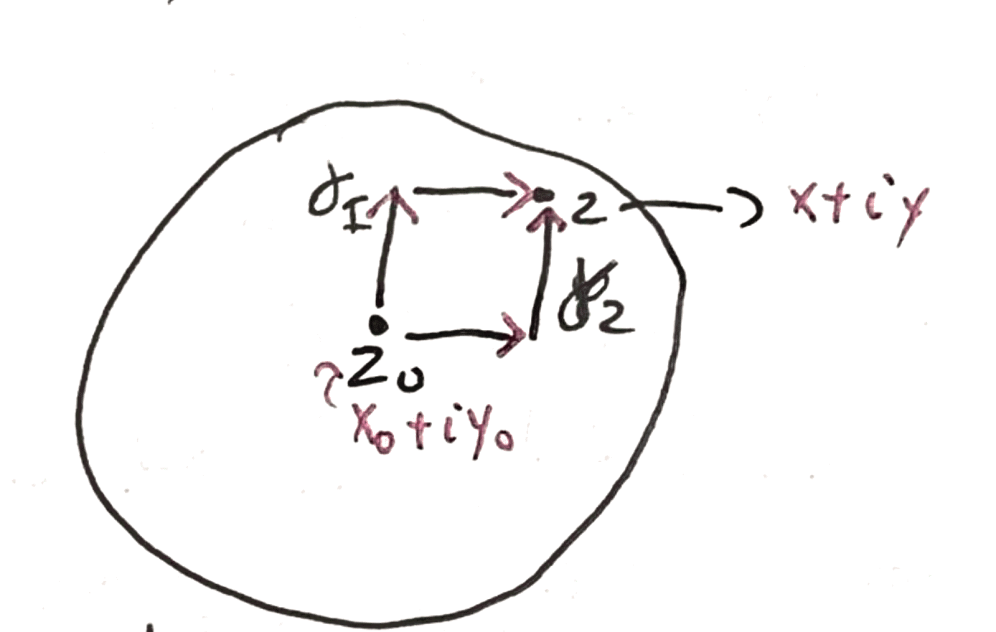
\includegraphics[width=.5\textwidth]{Figures/disk5.png}}\]
    For all $z \in \Omega$, define $F(z) = \int_{z_0}^z f(\xi) d\xi \coloneqq \int_{\gamma_1} f(z) dz = \int_{\gamma_2} f(z) dz$. We note that $F(z)$ is well-defined as Cauchy's Theorem guarantees the path-independence.\\\\
    \underline{We claim that $F \in CR^1(\Omega)$.} Indeed, tracing $\gamma_1$ and using the Fundamental Theorem of Calculus tells us that
    \[\frac{\partial F}{\partial x}(z) = f(z)\]
    Similarly, tracing along $\gamma_2$, we can parameterize $F(z)$ as
    \[F(z) = \int_{x_0}^x f(s + i y_0) ds + i \int_{y_0}^y f(x + it) dt\]
    Then it follows again that
    \[\frac{\partial F}{\partial y}(z) = i f(z)\]
    We can check that
    \[\frac{\partial F}{\partial x} + i \frac{\partial F}{\partial y} = f(z) - f(z) = 0\]
    , thus $F(z) \in CR^1(\Omega)$. Since $F(z)$ follows the Cauchy-Riemann Equations, we also know that
    \[F'(z) = \frac{1}{2}(\frac{\partial F}{\partial x} - i \frac{\partial F}{\partial y}) = \frac{1}{2}(2f(z)) = f(z)\]
    Since $F(z)$ is holomorphic, it is infinitely differentiable, so $f(z)$ is also holomorphic, so we are done.
\end{proof}

\begin{corollary}
    If $f_n \in C_z^1(\Omega)$ and $\{f_n\}$ converges to $f$ uniformly, then $f \in C_z^1(\Omega)$.
\end{corollary}

\begin{proof}
    For all sufficiently small rectangle $R$ within $\Omega$, consider
    \begin{align*}
        \int_{\partial R} f(z) dz &= \int_{\partial R} \lim_{n \to \infty} f_n dz\\
        &= \lim_{n \to \infty} \int_{\partial R} f_n dz \tag*{Uniform Convergence}\\
        &= \lim_{n \to \infty} 0 \tag*{Cauchy's Theorem}\\
        &= 0
    \end{align*}
    Thus, by Morera's Theorem, $f \in C_z^1(\Omega)$.
\end{proof}

\begin{corollary}
    If $f_n \in C_z^1(\Omega)$ and $\{f_n\}$ converges to $f$ uniformly, then $\{f_n'(z)\}$ converges to $f'(z)$ uniformly, and hence $\{f_n^{k}(z)\}$ converges to $f^{k}(z)$ uniformly.
\end{corollary}

\begin{proof}
It suffices for us to show this for the first derivative. Now for all $z \in \Omega$ and sufficiently small domain $G$, we have that
\begin{align*}
    f'(z) &= \frac{1}{2 \pi i} \int_{\partial G} \frac{f(z)}{(\xi - z)^2} d\xi \tag*{Cauchy's Formula for Derivatives}\\
    &= \frac{1}{2 \pi i} \int_{\partial G} \lim_{n \to \infty} \frac{f_n(z)}{(\xi - z)^2} d\xi\\
    &= \lim_{n \to \infty} \frac{1}{2 \pi i} \int_{\partial G} \frac{f_n(z)}{(\xi - z)^2} d\xi \tag*{Uniform Convergence}\\
    &= \lim_{n \to \infty} f_n'(z) \tag*{Cauchy's Formula for Derivatives}
\end{align*}
Thus, we have that $\{f_n'(z)\}$ converges to $f'(z)$. Since the original convergence is uniform, this convergence is also uniform.
\end{proof}

\begin{theorem}[Meta Theorem]
    Let $\phi(z, \xi): \Cbb \times X \to \Cbb$ where $X$ is some parameterization space with measure $\mu(\xi)$ that is finite, let
    $$f(z) = \int \phi(z, \xi) d\mu(\xi)$$
    Suppose $\phi$ is $CR^1$ in the variable $z$ and $f$ is bounded, then $f(z)$ is analytic.
\end{theorem}

\begin{proof}
    Since the measure $\mu$ is finite and the function is bounded, we can use Fubini's Theorem and see that, for all sufficiently small rectangles,
    \begin{align*}
        \int_R f(z) dz &= \int_R [\int \phi(z, \xi) d\mu(\xi)] dz\\
        &= \int [\int_R \phi(z, \xi) dz] d\mu(\xi) \tag*{Fubini's Theorem}\\
        &= \int 0 d\mu(\xi) \tag*{$\phi$ is $CR^1$ in the variable $z$}\\
        &= 0
    \end{align*}
\end{proof}

\begin{corollary}
    Let $f(z) = \sum_{n = 0}^\infty a_n (z - z_0)^n$ defined in $D_{z_0, r}$, then $f \in CR^1(D_{z_0, r}) = C_z^1(D_{z_0, r})$
\end{corollary}

\begin{proof}
    Let $z \in D(z_0, r)$, consider $r_1 > 0$ small enough that $cl(D(z, r_1)) \subset D(z_0, r)$, then by Heine-Cantor, we know that the partial sums
    \[\sum_{k = 0}^N a_k (z - z_0)^k \mapsto \sum_{0}^\infty a_n (z - z_0)^n \text{ converges uniformly in $D(z, r_1)$}\]
    Each of the partial sum are complex differentiable, thus by Corollary above, we have that $f \in C_z^1(D_{z_0, r})$.
\end{proof}

\begin{theorem}
    $CR^1 = C_z^1 = \text{Analytic}$
\end{theorem}

\begin{proof}
We have already shown all the directions in previous lectures and this lecture.
\end{proof}

\subsection{Power Series}

\begin{definition}
    Let $f(z) = \sum a_k (z - z_0)^k$ be a power series. We define the radius of convergence of $f$ as $R \in [0, \infty]$ such that for all $z$ such that $|z - z_0| < R$, $f(z)$ diverges, and for all $z$ such that $|z - z_0| > R$, $f(z)$ converges.
\end{definition}

\begin{remark}
    It turns out that
    \[\frac{1}{R} \coloneqq \lim \sup_{n \to \infty} |a_n|^{1/n}\]
\end{remark}

\begin{proposition}
    Let $f(z) = \sum a_k (z - z_0)^k$ be a power series with radius of convergence $R$, then $f(z)$ converges uniformly in any smaller disk of radius $r < R$ contained in $D_{z_0, R}$
\end{proposition}

\begin{proof}
    We note that $f$ is continuous on $D_{z_0, R}$, and the closure of any smaller disk is also contained in $D_{z_0, R}$, then apply Heine-Cantor.
\end{proof}

\begin{corollary}
    The following three power series:
    \begin{itemize}
        \item $\sum_{n = 0}^\infty a_n z^n$
        \item $\sum_{n = 0}^\infty n a_n z^{n-1}$
        \item $\sum_{n = 0}^\infty \frac{a_n}{n + 1} z^{n+1}$
    \end{itemize}
    all have the same radius of convergence.
\end{corollary}

\begin{proof}
    Exercise. Hint: Note that
    \[\lim_{n \to \infty} n^{1/n} = 1\]
\end{proof}

\begin{example}
    For sufficiently small $z \in \Cbb$, consider
    \[\frac{1}{1 + sin(z)} = 1 - sin(z) + sin^2(z) + ...\]
    , we can rewrite this into a power-series by noting that
    \[sin(z) = z - \frac{z^3}{3!} + \frac{z^5}{5!} + ...\]
\end{example}

\subsection{Liouville's Theorem}

\begin{theorem}
    Let $f \in Hol(\Cbb)$ be a holomorphic function on $\Cbb$, and for all $z \in \Cbb$ we have that $|f(z)| \leq M$ for some fixed $M \in \Cbb$, then $f(z)$ is identically constant.
\end{theorem}

\begin{proof}
Using Cauchy's Formula for Derivatives, we note that for all $z \in \Cbb$, for all $R > 0$,
\[f'(z) = \frac{1}{2\pi i} \int_{|\xi - z| = R} \frac{f(\xi)}{(\xi - z)^2} d\xi\]
Thus, we have that
\begin{align*}
    |f'(z)| \leq \frac{1}{2\pi} \max_{\xi \in |\xi - z|} |\frac{f(\xi)}{(\xi - z)^2}| \cdot 2 \pi R\\
    &\leq \frac{1}{2\pi} \frac{M}{R^2} \cdot 2 \pi R \tag*{Since $f$ is bounded}\\
    &= \frac{M}{R}
\end{align*}
Since this inequality holds for all $R > 0$, taking the limit as $R \to 0$, gives us that
\[|f'(z)| = 0\]
Hence $f'(z) = 0$, so
\[\frac{\partial f}{\partial z} = 0, \frac{\partial f}{\partial \overline{z}} = 0\]
So in other words
\[f_x - i f_y = 0, f_x + i f_y = 0 \implies f_x = 0, f_y = 0 \implies f(z) \text{ is constant}\]
\end{proof}

\begin{remark}
    While our Morera's Theorem applies to only triangles, up to a change of coordinate, the rectangle can really just be anything.
\end{remark}

\begin{remark}
    How to check say if $f(z) = |z|^2 = z \overline{z}$ is analytic or not? Well, we see that
    \[\frac{\partial f}{\partial \overline{z}} = \frac{\partial z}{\partial \overline{z}} \overline{z} + z \frac{\partial \overline{z}}{\partial \overline{z}} = 0 + z(1) \neq 0\]
    Thus, $f$ is not holomorphic and hence not analytic.\\\\
    Take another example, say $f(z) = |z| = (z \overline{z})^{1/2}$. This is real valued so we can use power rule and
    \[\overline{\partial}(f) = \frac{1}{2}(z \overline{z})^{-1/2} z \neq 0\]
\end{remark}

\subsection{Appendix - Cauchy–Hadamard Theorem}

In this section, we will discuss more about power series and convergence that was not covered during the lecture.

\begin{theorem}[Cauchy–Hadamard Theorem]
Consider $f(z) = \sum_{n = 0}^\infty a_n z^n$. Let $\frac{1}{0} = \infty$ and $\frac{1}{\infty} = 0$. Let $R$ be finite, non-zero, satisfying
\[\frac{1}{R} = \limsup |a_n|^{1/n}\]
Then $\sum_{n = 0}^\infty a_n z^n$ converges absolutely for $|z| < R$ and diverges for $|z| > R$. We call $R$ the \textbf{radius of convergence} and $|z| < R$ the \textbf{disc of convergence}.
\end{theorem}

% my attempt
\begin{proof}
For any $\epsilon > 0$, let $\rho \coloneqq \frac{1}{R}$.\\\\
If $|z| < R$, then there exist some $\epsilon > 0$ small enough that $|z| < \frac{1}{\rho + \epsilon} < \frac{1}{\rho} = R$. By the definition of $\limsup$ that for a sufficiently large $n$, for all $N > n$, 
\[|a_N|^{1/N} < \rho + \frac{\epsilon}{2} \ (*)\]
\begin{align*}
    |a_N z^N| &= |a_N^{1/N} z|^N\\
    &< |a_N^{1/N} \frac{1}{\rho + \epsilon}|^N \tag*{Since $|z| < \frac{1}{\rho + \epsilon}$}\\
    &< |\frac{\rho + \frac{\epsilon}{2}}{\rho + \epsilon}|^N \tag*{Using $(*)$}\\
\end{align*}
We note that $|\frac{\rho + \frac{\epsilon}{2}}{\rho + \epsilon}| < 1$ and $b_n = |\frac{\rho + \frac{\epsilon}{2}}{\rho + \epsilon}|^n$ forms a convergent geometric series. By the comparison test, we also have that $\sum_{n = N}^\infty a_n z^n$ converges, which implies that $\sum_{n = 0}^\infty a_n z^n$ converges.\\\\
If $|z| > R$, then there exist some $\epsilon > 0$ small enough that $|z| > \frac{1}{\rho - \epsilon} > \frac{1}{\rho} = R$. By the definition of $\limsup$ that for a sufficiently large $n$, for all $N > n$, 
\[|a_N|^{1/N} + \frac{\epsilon}{2} > \rho \ (*)\]
\begin{align*}
    |a_N z^N| &= |a_N^{1/N} z|^N\\
    &> |\frac{a_N^{1/N}}{\rho - \epsilon}|^N \tag*{Since $|z| > \frac{1}{\rho - \epsilon}$}\\
    &> |\frac{\rho - \frac{\epsilon}{2}}{\rho - \epsilon}|^N
\end{align*}
We note that $|\frac{\rho - \frac{\epsilon}{2}}{\rho - \epsilon}| > 1$ and $b_n = |\frac{\rho - \frac{\epsilon}{2}}{\rho - \epsilon}|^n$ forms a divergent geometric series, so the comparision test tells us that $\sum_{n = N}^\infty a_n z^n$ diverges, which implies that $\sum_{n = 0}^\infty a_n z^n$ diverges.
\end{proof}

\begin{corollary}\label{cor::radius_not_change}
Consider $f(z) = \sum_{n = 0}^\infty a_n z^n$ with radius of convergence $R > 0$, and let $g(z) = \sum_{n = 0}^\infty n a_n z^{n - 1}$. Then $g(z)$ has a radius of convergence that is also $R$.
\end{corollary}

\begin{proof}
Consider
\[\limsup_{n \to \infty} |n a_n|^{1/n} = \limsup_{n \to \infty} n^{1/n} |a_n^{1/n}|\]
It's a standard fact in real analysis that
\[\limsup_{n \to \infty} c_n b_n = \lim_{n \to \infty} c_n \limsup_{n \to \infty} b_n\]
if $\{c_n\}$ converges. We note that
\[\lim_{n \to \infty} n^{1/n} = 1\]
Since the limit exist
\[\limsup_{n \to \infty}  n^{1/n} |a_n^{1/n}| = \limsup_{n \to \infty} |a_n^{1/n}| = \frac{1}{R}\]
\end{proof}
\section{Lecture 6}

Previously, we have shown that a complex function $f: \Omega \to \Cbb$ is holomorphic if and only if it satisfies the Cauchy-Riemann Equations. Furthermore, if $f \in Hol(\Omega)$, $z_0 \in \Omega$, then we know $f$ is analytic and locally there exists some bounded, open set $G$ containing $z_0$ such that $\partial G$ is $PC^1$ $cl(G) \subset \Omega$, and on $G$,
\[f(z) = \sum_{k = 0}^\infty a_k (z - z_0)^k, |z - z_0| < r\]
\[a_n = \frac{1}{2 \pi i} \int_{\partial G} \frac{f(\xi)}{(\xi - z_0)^{n+1}} d\xi\]

\noindent Using the Cauchy's Formula for Derivatives, we note that
\[f^{(n)}(z_0) = \frac{n!}{2 \pi i} \int_{\partial G} \frac{f(\xi)}{(\xi - z_0)^{n+1}} d\xi \implies a_n = \frac{f^{(n)}(z_0)}{n!}\]

\subsection{Uniqueness Theorems}

\begin{theorem}
Let $f \in Hol(\Omega)$, $\Omega$ be an open and connected subset of $\Cbb$, and let $z_0 \in \Omega$ such that
\[f^{(n)}(z_0) = 0\ \forall n \geq 0\]
Then $f(z) = 0$ on $\Omega$, ie. $f$ is identically zero on $\Omega$.
\end{theorem}

\begin{proof}
We will prove this using \textbf{continuous induction}. Indeed, define $A$ to be the set
\[A \coloneqq \{z \in \Omega : f^{(n)}(z_0) = 0\ \forall n \geq 0\} = \bigcap_{n \geq 0} \{z \in \Omega: f^{(n)}(z) = 0\}\]
We first note that $A$ is closed since the preimage of $\{0\}$ is closed under continuous function and the intersection of closed sets are closed. Now clearly $A$ is non-empty, since $z_0 \in A$. We now \textbf{claim that $A$ is open}, then the connectedness of $\Omega$ would imply that $A = \Omega$.\\\\
Indeed, for all $z \in A$, since $f$ is holomorphic, we can find some $\epsilon(z) > 0$ small enough that locally
\[f(\xi) = \sum_{n = 0}^\infty \frac{f^{(n)}(z)}{n!}(\xi - z)^n, \forall \xi\ s.t.\ |\xi - z| < \epsilon\]
However, since $z \in A$, we know that
\[f(\xi) = \sum_{n = 0}^\infty \frac{0}{n!}(\xi - z)^n = 0\]
Thus we have that $\xi \in A$. Hence, $D_{z, \epsilon} \subset A$. Thus, $A$ is also open.
\end{proof}

\begin{remark}
The previous theorem shows that
\[f(z_0) = \sum a_n (z - z_0)^n, f^{(n)}(z_0) = 0\ \forall n \iff a_n = 0\ \forall n\]
\end{remark}

\begin{definition}[Limit Points]
Let $X$ be a topological space and $E \subset X$, we say $a \in X$ is a \textbf{accumulation/cluster/limit point} of $E$ if for all neighborhood $U$ containing $a$, $E \cap (U \setminus \{a\}) \neq \emptyset$
\end{definition}

\begin{theorem}[Uniqueness Theorem]\label{thm::uniqueness-theorem}
Let $f \in Hol(\Omega)$ where $\Omega$ is open and connected. Suppose $E \subset \Omega$ such that $f(z) = 0$ for all $z \in E$ and $E$ has some accumulation point $z_0$ in $\Omega$, then $f(z)$ is identically zero on $\Omega$.
\end{theorem}

\begin{proof}
The strategy is to apply the previous theorem. We first choose $r > 0$ small enough and consider the open disk $D_{z_0, r}$ to express $f$ as a power-series around $z_0$. Now, let $\Tilde{f}$ be $f$ restricted to $D_{z_0, r}$, we first claim that
\[\Tilde{f}(z_0) = 0\]
Indeed, since $z_0$ is a limit point of $E$, there exists a sequence of points $\{z_k\}$ in $E \cap D_{z_0, r}$ that converges to $z_0$. Since $f$ is continuous, we have that
\[\Tilde{f}(z_0) = \Tilde{f}(\lim_{k \to \infty} z_k) = \lim_{k \to \infty} \Tilde{f}(z_k) = \lim_{k \to \infty} 0 = 0\]
Now consider the power-series expression of $f$ around $z_0$:
\[[f(z) = \sum_{n = 0}^\infty a_n (z_0 - z)^n\]
Since $\Tilde{f}(z_0) = 0$, we clearly have that $a_0 = 0$. Now we will define
\[f_1(z) \coloneqq \frac{\Tilde{f}(z)}{z - z_0} = \sum_{n = 1}^\infty a_n (z - z_0)^{n-1}\]
\mattie{Division is fine here since $a_0 = 0$}
and define $\Tilde{f_1}(z)$ to be restricted to the same domain as before. Then clearly $f_1(z) = 0$ for all $z \in E \setminus \{z_0\}$, so it follows that $\Tilde{f_1}(z_0) = 0$, so $a_1 = 0$.\\\\
Using induction, we can conclude that all of the $a_n$ are $0$, so $f^{(n)}(z_0) = 0$ for all $n \geq 0$. Apply the previous result and we are done! 
\end{proof}

\begin{corollary}[Identity Theorem]
Let $f, g \in Hol(\Omega)$ where $\Omega$ is open and connected. Suppose $E \subset \Omega$ such that $f(z) = g(z)$ for all $z \in E$ and $E$ has some accumulation point $z_0$ in $\Omega$, then $f = g$ on $\Omega$.
\end{corollary}

\begin{proof}
Define $h(z) \coloneqq f(z) - g(z)$ and apply Theorem~\ref{thm::uniqueness-theorem}.
\end{proof}

\subsection{Analytic Extensions}

The uniqueness theorem implies that there's only one unique way to extend certain functions.

\begin{example}
Consider $f: \Rbb \to \Rbb$ given by $f(x) = e^x$, then $e^z = \sum_{n = 0}^\infty \frac{z^n}{n!}$ is an analytic extension of $e^x$ to the complex plane, and the identity theorem shows that it is in fact that only possible analytic extension.
\end{example}

\begin{proof}
Existence is already proven. For uniqueness, take $\Omega = \Cbb$ and $E = \Rbb$, $\Rbb$ clearly has an accumulation point in $\Cbb$, so we can apply the Identity Theorem.
\end{proof}

\begin{example}
Similarly, one can also show that
\[\cos(z) = 1 - \frac{z^2}{2!} + \frac{z^4}{4!} ...\]
\[\sin(z) = z - \frac{z^3}{3!} + \frac{z^5}{5!} ...\]
are the only unique extensions of $cos(x)$ and $sin(x)$, hence all trigonometric identities also hold for $z \in \Cbb$.
\end{example}

\begin{corollary}
Let $\Omega$ be an open connected set, suppose $f \in Hol(\Omega)$ isn't identically zero on $\Omega$, then the zeroes of $f$ are isolated.
\end{corollary}

\begin{proof}
Suppose not, then there exists a sequence of roots $\{z_k\}$ converging to some limit point. Then take $E = \{z_1, ..., z_k, ...\}$, then the Uniqueness Theorem tells us that $f$ is identically zero, so we have a contradiction.
\end{proof}

\begin{remark}
While this statement says that roots inside $\Omega$ are isolated, it says NOTHING about the boundary of $\Omega$.
\end{remark}

\subsection{Order of Zeroes}

\begin{definition}
Let $f \in Hol(\Omega)$, we define $Z(f)$ as the zero locus of $f$:
\[Z(f) \coloneqq f^{-1}(0)\]
\end{definition}

\begin{definition}
Suppose $f \in Hol(\Omega)$ and $f(z_0) = 0$, rewrite $f$ as a power series around $z_0$ as
\[f(z) = \sum_{n = 0}^\infty a_n (z - z_0)^n, a_0 = 0\]
We say the \textbf{order of zero} on $z_0$ is $\min \{n : a_n \neq 0\} = \min \{n: f^{(n)}(z_0) \neq 0$
\end{definition}

\begin{example}
$\sin(z)$ has zero of order $1$ at all roots. $(z - z_0)^3$ has a zero of order $3$ at $z_0$.
\end{example}
\section{Lecture 7}

\subsection{Revisiting Exponential}

\begin{definition}
    Let $z \in \Cbb$, we define the complex exponential map $e^z: \Cbb \to \Cbb$ as
    \[e^z \coloneqq 1 + z + \frac{z^2}{2!} + ... = \sum_{n = 0}^\infty \frac{z^n}{n!}\]
\end{definition}

\begin{theorem}[Euler's Identity]
Let $x \in \Rbb$, then
\[e^{ix} = cos(x) + i sin(x)\]
\end{theorem}

\begin{proof}
We can show this via explicit computation, indeed,
\begin{align*}
    e^{ix} &= \sum_{n = 0}^\infty \frac{(ix)^n}{n!}\\
    &= \sum_{k = 0}^\infty (-1)^k \frac{x^{2k}}{(2k)!} + i \sum_{k = 0} (-1)^k \frac{x^{2k + 1}}{(2k + 1)!} \tag*{Separate even and odd degree terms}\\
    &= cos(x) + i sin(x) \tag*{Taylor Series}
\end{align*}
\end{proof}

\begin{lemma}\label{lem::real_analy_fact}
Facts from Analysis:
\begin{enumerate}
    \item For every $r \in \Rbb$, $\sum_{n = 0}^\infty \frac{r^n}{n!}$ converges absolutely
    \item If $a_n \in \Cbb$ and $\sum_{n = 0}^\infty |a_n|$ converges, then $\sum_{n = 0}^\infty a_n$ converges
    \item If $L_a = \sum_{n = 0}^\infty a_n, L_b = \sum_{m = 0}^\infty b_m$ converges absolutely, then
    \[\sum_{n = 0}^\infty \sum_{k = 0}^n a_k b_{n - k}\]
    converges to
    \[(\sum_{n = 0}^\infty a_n) \cdot (\sum_{m = 0}^\infty b_m)\]
\end{enumerate}
This will helpful in proving some identities.
\end{lemma}

\begin{proof}
For $(1)$, we will use the ratio test. Indeed, consider $a_n = \frac{r^n}{n!}$, then
\[\lim_{n \to \infty} |\frac{a_{n+1}}{a_n}| = \lim_{n \to \infty} |\frac{r}{n + 1}| = 0 < 1\]
Thus, the series converges absolutely.\\\\
For $(2)$, let $b_n = \sum_{i = 1}^n a_i, c_n = \sum_{i = 1}^n |a_i|$. We note that the topology $\Cbb$ is homeomorphic to the Euclidean topology on $\Rbb^2$, so in particular $\Cbb$ is a complete metric space, so a sequence is convergent if and only if it is Cauchy. We know $c_n$ converges, so for every $\epsilon > 0$, there exists some $N_c$ such that for all $i, j > N_c$.
\[|c_i - c_j| < \epsilon\]
It remains for us to show that $b_n$ is also Cauchy. Indeed, if $i = j$, then we are done. Without loss, we will then assume $j > i$, then
\begin{align*}
    |b_i - b_j| &= |\sum_{k = i + 1}^j a_k|\\
    &\leq \sum_{k = i + 1}^j |a_k| \tag*{Triangle's Inequality}\\
    &= |c_i - c_j|\\
    &< \epsilon
\end{align*}
Thus, $\{b_n\}$ is Cauchy and converges.\\\\
For $(3)$, $(\sum_{n = 0}^\infty a_n) \cdot (\sum_{m = 0}^\infty b_m)$ certainly converges to $L_a \cdot L_b$. Now write $(\sum_{n = 0}^\infty a_n) \cdot (\sum_{m = 0}^\infty b_m) = \sum_{n = 0}^\infty \sum_{m = 0}^\infty a_n b_m$, this corresponds exactly to the terms of $\sum_{n = 0}^\infty \sum_{k = 0}^n a_k b_{n - k}$. The exact combinatorics is left as details to the reader.
\end{proof}

\begin{corollary}
Let $e^z$ be the complex exponential map, then
\begin{itemize}
    \item $e^z$ converges for all $z \in \Cbb$
    \item $e^{z + w} = e^z \cdot e^w$ for all $z, w \in \Cbb$
\end{itemize}
\end{corollary}

\begin{proof}
For the first, let $a_n = \sum_{k = 1}^n |\frac{z^k}{k!}|$. It suffices for us to prove that $a_n$ converges as absolute convergence implies monotone convergence from Lemma~\ref{lem::real_analy_fact}(2). But we note that 
\[|\frac{z^k}{k!}| = \frac{|z|^k}{k!}\]
and $|z|$ is a real number, so Lemma~\ref{lem::real_analy_fact}(1) tells us that $a_n$ converges.\\\\
For the second, we note that
\begin{align*}
    e^{z + w} &= \sum_{n = 0}^\infty \frac{(z + w)^n}{n!}\\
    &= \sum_{n = 0}^\infty \sum_{k = 0}^n {n \choose k} \frac{z^k w^{n-k}}{n!} \tag*{Binomial Theorem}\\
    &= \sum_{n = 0}^\infty \sum_{k = 0}^n \frac{z^k}{k!} \frac{w^{n-k}}{(n - k)!}\\
    &= (\sum_{n = 0}^\infty \frac{(z)^n}{n!}) \cdot (\sum_{n = 0}^\infty \frac{(w)^n}{n!}) \tag*{By Lemma~\ref{lem::real_analy_fact}(3)}\\
    &= e^z \cdot e^w
\end{align*}
\end{proof}

\begin{proposition}
We can also recover $\cos(z)$ and $\sin(z)$ from $e^z$ as
\[\cos(z) = \frac{e^{iz} + e^{-iz}}{2}, \sin(z) = \frac{e^{iz} - e^{-iz}}{2i}\]
If $x \in \Rbb$, we also have that
\[\cos(x) = \Re e^{ix}, \sin(x) = \Im e^{ix}\]
\end{proposition}

\subsection{Complex Logarithms}

As in the case of $\Rbb$, we want to define $\log(z)$ as an inverse to $e^z$ such that
\[e^{\log(z)} = z\]
The problem is that $e^z$ is not actually injective, so there are multiple choices for $\log(z)$. Consequently, this will result in $\log(z)$ not being continuous on all of $\Cbb$.

\begin{question}
Given $z$, can we find all solutions satifying $e^w = z$?
\end{question}

\begin{proof}[Answer]
We will again leverage on Polar Coordinates. Indeed, write $z = re^{i \theta}, w = x + iy$, then we have that
\[r e^{i \theta} = e^{x + iy} = e^{x} e^{iy}\]
Thus, $x = \log(r), y = \theta + 2 \pi k$.\\\\
Thus, $w$ is of the form $w_k = \log(r) + i(\theta + 2 \pi k)$
\end{proof}

\begin{definition}[Complex Logarithm]
    For $z \in \Cbb \setminus \{0\}$, write $z = re^{i \theta}, \theta \in [-\pi, \pi]$. Then we define
    \[\log(z) = \log(r e^{i \theta}) \coloneqq \log(r) + i \theta\]
    $\theta$ is sometimes refered to as the \textbf{principal argument} of $z$ and we denote $Arg(z) = \theta$.
\end{definition}

\begin{remark}
Note that the complex logarithm $\log(z)$ is not continuous on all of $\Cbb$:
\[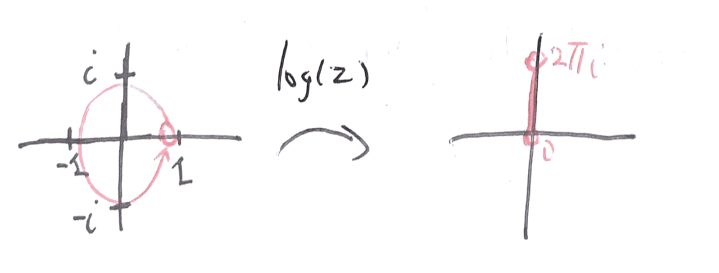
\includegraphics[width=0.5\textwidth]{Figures/complex_log.png}\]
As you trace around the unit circle, going back to $z = 1$ presents a problem.\\\\
Therefore, we can only define the complex logarithm up to a \textbf{branch cut} that's a radial line extending out from the origin. We will without loss choose this branch to be $(-\infty, 0]$
\end{remark}

\begin{proposition}
$\log(z)$ is holomorphic on $\Cbb \setminus (-\infty, 0]$ and in fact $\frac{d}{dz} \log(w) = \frac{1}{w}$
\end{proposition}

\begin{proof}
One way to do this is to use the Cauchy-Riemann equations in polar coordinates. We will however use the Inverse Function Theorem instead. Indeed, we note that on $\Cbb \setminus (-\infty, 0]$, $z \mapsto e^z$, when viewed as a function from $\Rbb^2$ to $\Rbb^2$, is a smooth function whose derivative is exactly
\[(e^z)' = e^x \begin{pmatrix} cos(y) & -sin(y)\\ sin(y) & cos(y) \end{pmatrix}\]
, which satisfies the matrix representation of complex numbers (hence we can extend the argument to holomorphic functions). Thus, the inverse function theorem tells us that $g(z) = \log(z)$ is also holomorphic and that
\[g'(f(x)) = (f'(x))^{-1}\]
This equation tells us that, locally for all $w = e^z \in \Cbb \setminus (-\infty, 0]$,
\[\frac{d}{dz} \log(w) = e^{-x}\begin{pmatrix} cos(y) & sin(y)\\ -sin(y) & cos(y) \end{pmatrix} = (e^{z})^{-1} = \frac{1}{w}\]
Note that the branch cut does not prevent the existence of a local inverse, but it does prevent the existence of a global inverse on all of $\Cbb$.
\end{proof}

\begin{remark}
Let $z \in \Cbb \setminus (-\infty, 0]$, then since $\frac{1}{z}$ is primitive on the path $1$ to $z$, we have that:
\[\int_1^z \frac{d\xi}{\xi} = \log(z) - \log(1) = \log(z)\]
\end{remark}

\subsection{Homotopy Invariance of Integral}

Let $f \in Hol(\Omega)$ and $\gamma: [a, b] \to \Gamma$ is continous and $\Gamma \subset \Omega$, then we can define the integral
\[\int_\gamma f(z) dz\]

Informally, we can define this because at each point on $\gamma$, we can find some disk to represent $f$ as a power series with a primitive $F$, then we can split $[a, b]$ into a union of (not necessarily uniform) subintervals, then the integral $\gamma$ can be approximated as a sum of the anti-derivatives $F_k$ at each end-points.

We can formally justify this with what's called the Lebesgue's Number Lemma.

\begin{lemma}[Lebesgue's Number Lemma]
Let $K$ be a compact metric space and let $\{U_a\}$ be an open cover for $K$, then there exists some $\delta > 0$ (we call the \textbf{Lebesgue Number}) such that for all $x \in K$, there exists some $a$ such that $B_{x, \delta} \subset U_a$
\end{lemma}

\begin{proof}
For all $x \in K$, since $\{U_a\}$ is an open cover of $K$, there exists some $a$ such that $x \in U_a$. Since $U_a$ is open, there exists some $r(x) > 0$ small enough such that $B_{x, 2r(x)} \subset U_\alpha$.\\\\
Note that $\{B_{x, r(x)}\}$ running over all $x \in K$ is an open cover of $K$. Since $K$ is compact, we in fact have a finite subcover:
\[B_{x_1, r_1}, ..., B_{x_n, r_n}\]
Choose $\delta = \min \{r_i\}$. Now for all $x \in K$, it belongs to one of the $B_{x_k, r_k} \subset U_a$.\\\
Then we claim $x \in B_{x, \delta} \subset B_{x_k, 2r_k} \subset U_a$. To do this, we need to verify $B_{x, \delta} \subset B_{x_k, 2r_k}$. Indeed, for all $y \in B_{x, \delta}$, we have that
\[d(y, x_k) \leq d(y, x) + d(x, x_k) < \delta + r_k \leq 2r_k\]
This concludes the proof.
\end{proof}

To apply this lemma in our context, we take $K = [a, b]$ and for all $s \in [a, b]$, we define $U_s = \gamma^{-1}(D_{\gamma(s), r(s)})$, where $r(s)$ is the radius of convergence of $\gamma(s)$ under the power-series. Then we can apply the Lebesgue's Number Lemma.

\begin{question}
Is the integral well-defined up to two different splitting?
\end{question}

\begin{proof}[Answer]
Yes, the idea is that given two splitting on the interval, one can join them using a refinement by taking smaller intervaks of both of them and used the associated anti-derivative from either original splittings. To be more rigorous, let $\{I_k\}$ and $\{J_n\}$ be two different splittings of the interval $[0, 1]$. Now define
\[I_{k, n} \coloneqq I_k \cap J_n\]
Then we note that, by definition, the integral over the splitting $I_{k, n}$ would be of the form
\begin{align*}
    \sum \int_{I_{k, n}} f(z) dz &= \sum_{k} \sum_{n} \int_{I_{k, n}} f(z) dz\\
    &= \sum_k [\sum_{n} \int_{I_{k, n}} f(z) dz]\\
    &= \sum_k \int_{I_k} f(z) dz
\end{align*}
Similarly, we can also show that
\[\sum \int_{I_{k, n}} f(z) dz = \sum_n \int_{J_n} f(z) dz\]
Thus, the two splittings yield the same integral.
\end{proof}

\begin{definition}
    Let $\gamma_0, \gamma_1: [a, b] \to \Omega$ be continuous. We say $\gamma_0$ is \textbf{homotopy equivalent} to $\gamma_1$ if there exists a continuous function $\Gamma: [a, b] \times [0, 1] \to \Omega$ such that $\Gamma(s, 0) = \gamma_0(s)$ and $\gamma(s, 1) = \gamma_1(s)$ for all $s \in [a, b]$.\\
    We will also assume that either:
        \begin{itemize}
            \item All pathes are closed, for all $t$
            \[\Gamma(a, t) = \Gamma(b, t)\]
            \item OR Endpoints are fixed
            \[\Gamma(a, t) = \gamma_0(a) = \gamma_1(b)\]
            \[\Gamma(b, t) = \gamma_0(b) = \gamma_1(b)\]
        \end{itemize}
\end{definition}

\begin{theorem}
If $\gamma_0, \gamma_1$ are homotopy equivalent in $\Omega$ and $f \in Hol(\Omega)$, then
\[\int_{\gamma_0} f(z) dz = \int_{\gamma_1} f(z) dz\]
\end{theorem}

\begin{remark}
In a simply connected domain, any two pathes are homotopy equivalent. In otherwords, the path of integration is irrelevant.
\end{remark}
\section{Lecture 8}

\subsection{Homotopy Invariance of Integrals - Continued}

\begin{theorem}
If $\gamma_0, \gamma_1$ are homotopy equivalent in $\Omega$ and $f \in Hol(\Omega)$, then
\[\int_{\gamma_0} f(z) dz = \int_{\gamma_1} f(z) dz\]
\end{theorem}

\begin{proof}
Let $\Gamma$ be the homotopy equivalence function. For all $z_0 \in \Omega$, let $D_{z_0}$ be a disc centered at $z_0$ small enough such that $f$ can be expressed as a power-series on it, define
\[U_{z_0} = \Gamma^{-1}(D_{z_0})\]
Then $\{U_{z_0}\}$ will be an open cover of $R \coloneqq [a, b] \times [0, 1]$, which is a compact metric space. Apply Lebesgue's Number Lemma, we find $\delta > 0$ such that, we can split $R$ into smaller rectangles $R_k$ where each $diam(R_k) < \delta$.\\\\
The Lebesgue Number Lemma tells us that, for each $R_k$, $\Gamma(cl(R_k)) \subset D_{z}$ for some $z$. Since $f$ is primitive on $D_z$, we have that
\[\int_{\Gamma|_{\partial R_k}} f(z) dz = 0\]
Putting the small rectangles together (Green's Theorem style), the inner edges cancel out, so we have that
\[\int_{\Gamma|_{\partial R}} f(z) dz = 0\]
Now consider the pathes $\ell_1 = \{a\} \times [0, 1]$ and $\ell_2 = \{b\} \times [0, 1]$, we claim that
\[\int_{\Gamma|_{\ell_1 + \ell_2}} f(z) dz = 0\]
Indeed, if endpoints are fixed, both paths are constant (stays at same point). If all path are closed, then this is the same path in opposite directions.\\\\
Thus, we only have to integrate over the horizontal pathes:
\[\int_{\partial R} f(z) dz = 0 = \int_{\gamma_0} f(z) dz - \int_{\gamma_1} f(z) dz\]
\end{proof}

\begin{definition}
    A set $\Omega$ is \textbf{simply connected} if any closed loop in $\Omega$ is homotopy equivalent to the constant path. This is equivalent to saying, for any pathes $\gamma_0, \gamma_1$, $\gamma_0(a) = \gamma_1(a) = z_0$, $\gamma_0(b) = \gamma_1(b) = z_1$, are homotopy equivalent.
\end{definition}

\begin{remark}
If $\Omega$ is simply connected domain, then
\[\int_{z_0}^z_1 f(z) dz\]
does not depend on the path specified.
\end{remark}

\begin{definition}
    Let $\Omega$ be simply connected and $f \in Hol(\Omega)$. Suppose $f(z) \neq 0$ for all $z \in \Omega$.\\\\
    Fix some $z_0 \in \Omega$, and consider
    \[a_0 \text{ such that } f(z_0) = e^{a_0}\]
    We can find $a_0$ as
    \[Re(a_0) = \log |f(z_0)|, Im(a_0) = arg\ f(z_0)\]
    Then we define
    \[\log f(z) \coloneqq a_0 + \int_{z_0}^z \frac{f'(\xi)}{f(\xi)} d\xi\]
\end{definition}

Show that $\log f(z)$ aligns with the global definition of the complex logarithm.

\begin{proof}
Exercise. The idea is to denote $\varphi(z) = a_0 + \int_{z_0}^z \frac{f'(\xi)}{f(\xi)} d\xi$ and show that
\[(f(z) e^{-y(z)})' = 0\]
and realize that their product must be $1$.
\end{proof}

\mattie{explain motivation later}
\begin{definition}
    What is $f(z)^{\alpha}$? We define
    \[f(z)^{\alpha} = e^{\alpha \log(f(z))}\]
    This is defined when $f \in Hol(\Omega)$, $f(z) \neq 0$ on all of $\Omega$, and $\Omega$ is simply connected.
\end{definition}

In a simply connected domain, the branch of the logarithm, it is enough to be determined by which $a_0$ you choose.

\subsection{Laurent Series}

Suppose $f$ is holomorphic on $\{z : a < |z - z_0| < A\}$, where we require $a \geq 0$ and $A \leq \infty$.

\begin{theorem}
If $f \in Hol\{z : a < |z - z_0| < A\}$, then $f$ can be represented as
\[f(z) = \sum_{n \in \Zbb} a_n (z - z_0)^n\]
, where we have that
\[a_n = \frac{1}{2\pi i} \int_{|\xi - z_0| = r} f(\xi) (\xi - z_0)^{-(n+1)} d\xi\]
, where $r$ is between $a < r < A$ (Note that for $\Zbb_+$, this is the same as the Taylor Power Series)
\end{theorem}

\begin{proof}
Without loss of generality, we can shift this to $z_0 = 0$.\\\\
Take $z$ such that $a < |z| < A$ and pick $r, R$ such that
\[a < r < |z| < R < A\]
Then consider the set
\[G \coloneqq \{z: r < |z| < R \}\]
Then Cauchy's Integral Formula gives
\begin{align*}
    f(z) &= \frac{1}{2\pi i} \int_{\partial G} \frac{f(\xi)}{\xi - z} d\xi\\
    &= \frac{1}{2\pi i} (\int_{|z| = R} \frac{f(\xi)}{\xi - z} d\xi - \int_{|z| = r} \frac{f(\xi)}{\xi - z} d\xi)\\
    &= \frac{1}{2\pi i} (I_1 - I_2)
\end{align*}
For $I_1$, we note that $|z| < |\xi| = R$, so
\begin{align*}
    I_1 &= \int_{|z| = R} \frac{f(\xi)}{\xi - z} d\xi\\
    &= \int_{|z| = R} \frac{f(\xi)}{\xi} \frac{1}{1 - \frac{z}{\xi}} d\xi\\
    &= \int_{|z| = R} f(\xi) \sum_{k = 0}^\infty \frac{z^k}{\xi^{k+1}}
\end{align*}
For $I_2$, we note that $|z| > |\xi| = r$, so
\begin{align*}
    I_2 &= \int_{|z| = r} \frac{f(\xi)}{\xi - z} d\xi\\
    &= \int_{|z| = r} \frac{-f(\xi)}{z} \frac{1}{1 - \frac{\xi}{z}} d\xi\\
    &= \int_{|z| = r} -f(\xi) \sum_{k = 0}^\infty \frac{\xi^k}{z^{k+1}}\\
    &= \int_{|z| = r} -f(\xi) \sum_{n = -\infty}^{-1} \frac{z^n}{\xi^{n+1}}\\ \tag*{Change of Variables}
\end{align*}
Since both series converge uniformly, we can integrate term by term and use Cauchy's Formula for Derivatives, rewriting both $I_1$ and $I_2$ out in series finishes the proof.
\end{proof}

Now we will consider a particular case of the Laurent Series!

\begin{definition}
    Let $f \in Hol(\Omega \setminus \{z_0\})$ where $z_0 \in \Omega$. In this case, we say $f$ has a singularity at $z_0$.\\\\
    Take $\delta$ small enough and $D_{z_0, \delta} \subset \Omega$, then the Laurent Series tells us
    \[f(z) = \sum_{n \in \Zbb} a_n (z - z_0)^n\]
    We say that
    \begin{itemize}
        \item $f$ has a \textbf{removable singularity} at $z_0$ if $a_n = 0$ for all $n < 0$. In this case,
        \[f(z) = \sum_{n \geq 0} a_n (z - z_0)^n, f(z_0) = a_0\]
        An example of such function would be $f(z) = \frac{sin(z)}{z}$ has removable singularity at $0$
        \item We say $f$ has a \textbf{pole at $z_0$} if $a_n \neq 0$ for finitely many $n < 0$. We say the \textbf{order of a pole} as
        \[\max \{n \geq 0: a_{-n} = 0\}\]
        \item We say that $f$ has an essential singularity if there exists infinitely many $n < 0$ such that $a_n \neq 0$.\\\\
        For example consider
        \[f(z) = e^{1/z} = \sum_{n = 0}^\infty \frac{z^{-n}}{n!}\]
        This has an essential singularity at $z = 0$.
    \end{itemize}
    These are the singularities we care about.
\end{definition}
\section{Lecture 9}

\subsection{Classification of Singularities}

Recall, let $f \in Hol(\Omega \setminus \{z_0\})$, where $z_0 \in \Omega$, we can write $f$ into a Laurent series
\[f(z) = \sum_{z \in \Zbb} a_n (z - z_0)^n, 0 < |z - z_0| < N\]
, and we say that $z_0$ is removable if $a_n = 0$ for all $n < 0$.

\begin{theorem}
$z_0$ is a removable singularity of $f$ if and only if there exists a neighborhood $z_0 \in U$ such that $f$ is bounded in $U \setminus \{z_0\}$.
\end{theorem}

\begin{proof}
If $f$ has a removable singularity, we can write it locally as
\[f(z) = \sum_{n \geq 0} a_n (z - z_0)^n\]
which has a positive radius of convergence and hence bounded in a neighborhood of $z_0$.\\\\
Conversely, suppose $f$ is bounded on $0 < |z - z_0| < \delta$. Then for all $n \geq 1$, we note that
\[a_{-n} = \frac{1}{2\pi i} \int_{|z - z_0| = r} f(z) (z - z_0)^{n-1} dz \]
As $n-1 \geq 0$ and $f$ is bounded, this integral is also bounded, so
\[|a_{-n}| \leq \frac{1}{2\pi} M (1) (2\pi r) = Mr\]
for all $0 < r < \delta$, we can shrink $r$ down and have that $a_{-n} = 0$.
\end{proof}

\begin{remark}
If $f(z) = o(\frac{1}{|z - z_0|})$, then $f$ has a removable singularity at $z_0$.
\end{remark}

We say $f$ has a \textbf{pole at $z_0$} if $a_n \neq 0$ for finitely many $n < 0$. We say the \textbf{order of a pole} as
        \[\max \{n \geq 0: a_{-n} = 0\}\]
        
\begin{theorem}
$z_0$ is a pole if and only if $\lim_{z \to z_0} |f(z)| = \infty$
\end{theorem}

\begin{proof}
Suppose $z_0$ is a pole of order $m$, then we can write
\[f(z) = \frac{g(z)}{(z - z_0)^m}, g(z_0) \neq 0\]
Hence we have that
\[\lim_{z \to z_0} |f(z)| = \lim_{z \to z_0} |\frac{g(z)}{(z - z_0)^m}| = \infty\]
Conversely, suppose $\lim_{z \to z_0} |f(z)| = \infty$, then we can find some $r > 0$ such that $|f(z)| > 1$ for all $z$ in $0 < |z - z_0| < r$.\\\\
Now consider $h(z) = \frac{1}{f(z)}$ on $D_{z_0, r} \setminus \{z_0\}$, then $h(z) \in Hol(D_{z_0, r} \setminus \{z_0\})$ and $\lim_{z \to z_0} h(z) = 0$ - so we can extend $h$ to the whole disk. Therefore it has to be the case that $|h(z)| < 1$, then by the previous theorem, this means $z_0$ is a removable singularity for $h$, so in fact $h$ is holomorphic on the whole disk.\\\\
Since $h(z_0) = 0$, we can find the smallest $m$ such that $h(z) = (z - z_0)^m h_0(z)$ but $h_0(z_0) \neq 0$. Now consider $g = \frac{1}{h}$, then we have that
\[f(z) = \frac{g(z)}{(z - z_0)^m}\]
Thus, $z_0$ is a pole of order $m$.
\end{proof}

We say that $f$ has an essential singularity if there exists infinitely many $n < 0$ such that $a_n \neq 0$.

\begin{theorem}[Casorati-Weierstrass Theorem]
If $f$ has an essential singularity at $z_0$, then for any neighborhood $U$ of $z_0$, $U \subset \Omega$, $f(U)$ is \textbf{dense} in $\Cbb$ (in other words, for all $w \in \Cbb$, there exists a sequence of $z_n$ such that $f(z_n) \to w$ as $z_n \to z_0$)
\end{theorem}

\begin{proof}
We will prove this using contradiction. Suppose there exists some neighborhood $U$ of $z_0$ such that $f(U)$ is not dense. Then there exists some $a \in \Cbb$ and $r > 0$ such that $D_{a, r} \cap f(U) = \emptyset$.\\\\
Now define $g(z) = \frac{1}{f(z) - a}$. Then clearly $g \in Hol(U)$ as the denominator is never $0$. We also have that $|g| < \frac{1}{|f(z) - a|} < \frac{1}{r}$. Moreover, we note that $g(z) \neq 0$ in $U \setminus \{z_0\}$ because $f$ is bounded. While $g(z_0)$ could be $0$, we will choose the smallest $m$ such that $g(z) = (z - z_0)^m g_0(z)$ and $g_0(z_0) \neq 0$.\\\\
Thus, $g_0(z) \neq 0$ on $U$. But we have that
\[f(z) = \frac{1}{g(z)} + a = \frac{1}{(z - z_0)^m g_0(z)} + a\]
, so $f$ has a removable singularity or some pole at $z_0$, hence a contradiction.
\end{proof}

\begin{definition}
    Suppose $f$ has a singularity at $z_0$ and write
    \[f(z) = \sum_{n \in \Zbb} a_n (z - z_0)^n\]
    Then we define the \textbf{residue of $f$ at $z_0$} as $a_{-1}$ and denote is as $Res_{z_0}(f)$ or $res(f, z_0)$
\end{definition}

\begin{remark}
If $z_0$ is a pole of order $1$, then
\[res(f, z_0) = \lim_{z \to z_0} (z - z_0)f(z)\]
\end{remark}

\subsection{Cauchy's Residue Theorem}

\begin{theorem}[Cauchy's Residue Theorem]
Let $G$ be a bounded domain with $\partial G \in PC^1$ and $\overline{G} \subset \Omega$. Let $z_1, ..., z_n \in G$ and $f \in Hol(\Omega \setminus \{z_1, ..., z_n\})$, then
\[\int_{\partial G} f(z) dz = 2\pi i \sum_{k = 1}^n Res(f, z_k)\]
\end{theorem}

\begin{proof}
Let $D_k$ be small disks around each $z_k$ and consider $\Tilde{G} = G \setminus \bigcup D_k$. Note that $f(z)$ is holomorphic on $\Tilde{G}$, so
\[\partial_{\partial \Tilde{G}} f(z) dz = 0\]
On the other hand, we also have that $\partial \Tilde{G} = \partial G - \bigcup \partial D_k$, so in other words
\[\int_{\partial G} f(z) dz = \sum_k \int_{\partial D_k} f(z) dz\]
Write $f$ as a Laurent Series, then every term except for the $-1$ term is primitive and thus evaluate to $0$, so we are left with:
\[\int_{\partial G} f(z) dz = 2\pi i \sum_{k = 1}^n Res(f, z_k)\]
\end{proof}
\section{Lecture 10 - 09/28/2022}

Clarification from last lecture: In the proof of the Casorati–Weierstrass theorem, we have that $g(z) \neq 0$ for all $z \in U\setminus \{z_0\}$, but $g(z_0) = 0$ is totally possible! Hence we write
\[f(z) = \frac{1}{g(z)} + a\]
, where $f$ either has a pole or a removable singularity at $z_0$, giving the contradiction.

\subsection{Computing Real Integrals with Residues}

\begin{example}[A Straight-forward Application]
Let $s \in \Rbb$, consider the integral
\[I = \int_{-\infty}^\infty \frac{1}{x^2 + 1} e^{isx} dx\]
Let $f(z) = \frac{1}{x^2 + 1} e^{isx}$, then $I = \int_{\Rbb} f(z) dz = \pi e^{-|s|}$
\end{example}

\begin{remark}
Why do we even care about integrals of this form? Well, they are really closed aligned with \textbf{inverse Fourier transforms}. In particular, you would calculate integrals of the form
\[F(s) = \int_{-\infty}^\infty f(x) e^{-2\pi i s} dx\]
\end{remark}

\begin{proof}[Proof of Example]
We will consider three cases $s = 0, s > 0,$ and $s < 0$. For $s = 0$, this is obvious.\\\\
Now for $s > 0$, consider the following contour:
\[\fbox{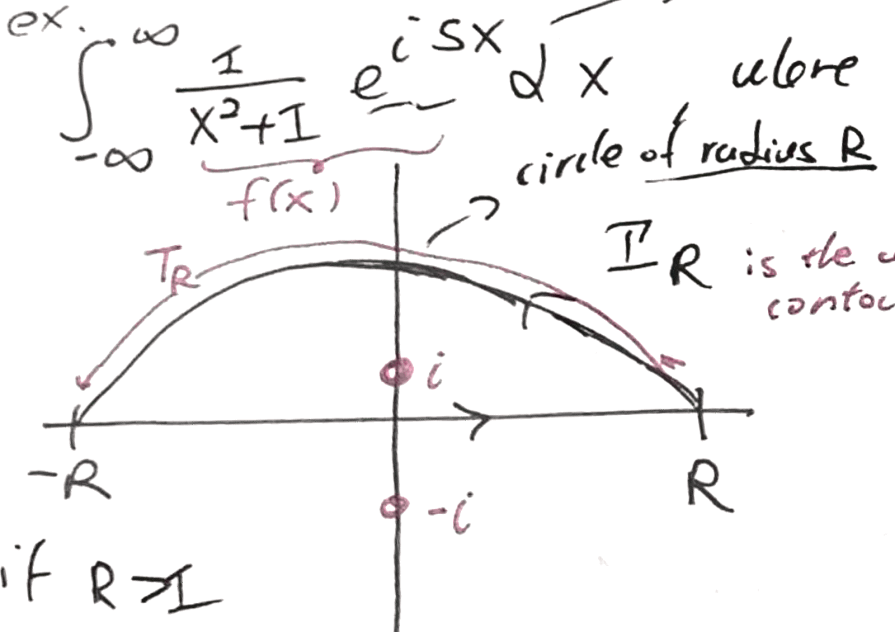
\includegraphics[width=.5\textwidth]{Figures/contour-1.png}}\]
Then Cauchy's Residue Theorem tells us that
\[\int_{\Gamma_R} f(z) dz = 2 \pi i Res(f, i)\]
$i$ is a pole of order $1$ for $f$, so
\[Res(f, i) = \lim_{z \to i} (z -i)f(z) = \frac{e^{-s}}{2i}\]
Thus, we have that
\[\int_{\Gamma_R} f(z) dz = \pi e^{-s}\]
Now take $R \to \infty$, we note that since \textbf{$f$ is integrable} as $\int_{-\infty}^\infty |f(x)| dx < \infty$,
\[\lim_{R \to \infty} \int_{-R}^R f(z) dz = \int_{-\infty}^{\infty} f(z) dz = I\]
So in other words,
\[I = \lim_{R \to \infty} [\int_{\Gamma_R} f(z) dz - \int_{T_R} f(z) dz] = \pi e^{-s} - \lim_{R \to \infty} \int_{T_R} f(z) dz\]
We want to show that the last term goes to $0$, indeed
\begin{align*}
    \int_{T_R} f(z) dz &= \int_0^\pi \frac{e^{isRe^{it}}}{(Re^{it})^2 + 1} i Re^{it} dt \tag*{Let $z = R e^{it}$}\\
    |\int_{T_R} f(z) dz| &\leq \frac{R}{R^2 - 1} \pi \tag*{Note that $e^{isRe^{it}}$ is bounded by $1$ as $s > 0$ and $0 < t < \pi$}
\end{align*}
Taking $R \to \infty$, the bound goes to $0$, thus, we have that
\[I = \pi e^{-s}, s \geq 0\]
\textbf{What about when $s < 0$}? In this case, $\int_{T_R} f(z) dz$ would not actually go to $0$, so instead, we need to consider the opposite contour:
\[\fbox{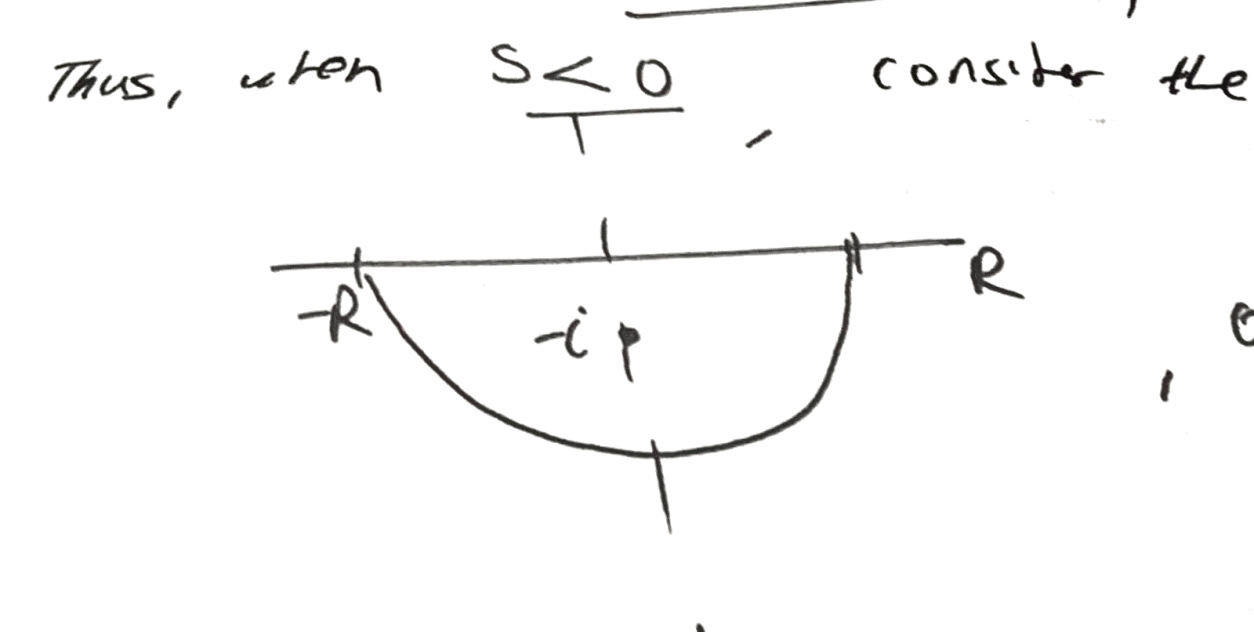
\includegraphics[width=.5\textwidth]{Figures/contour-2.png}}\]
, and we can similarly show the result is true. Alternatively, we could also have argued using symmetry.\\\\
Note that while we proved this using a circle, we could have also used a rectangle instead.
\end{proof}

\begin{example}[A Not-So-Simple Application]
Let $s \in \Rbb$ and $a \in \Cbb$ such that $s > 0$ and $\Im(a) > 0$, consider the integral
\[I = \int_{-\infty}^\infty \frac{e^{isx}}{x - a} dx\]
Let $f(z) = \frac{e^{isz}}{z - a}$, then what is $I$?
\end{example}

Consider the following contour:
\[\fbox{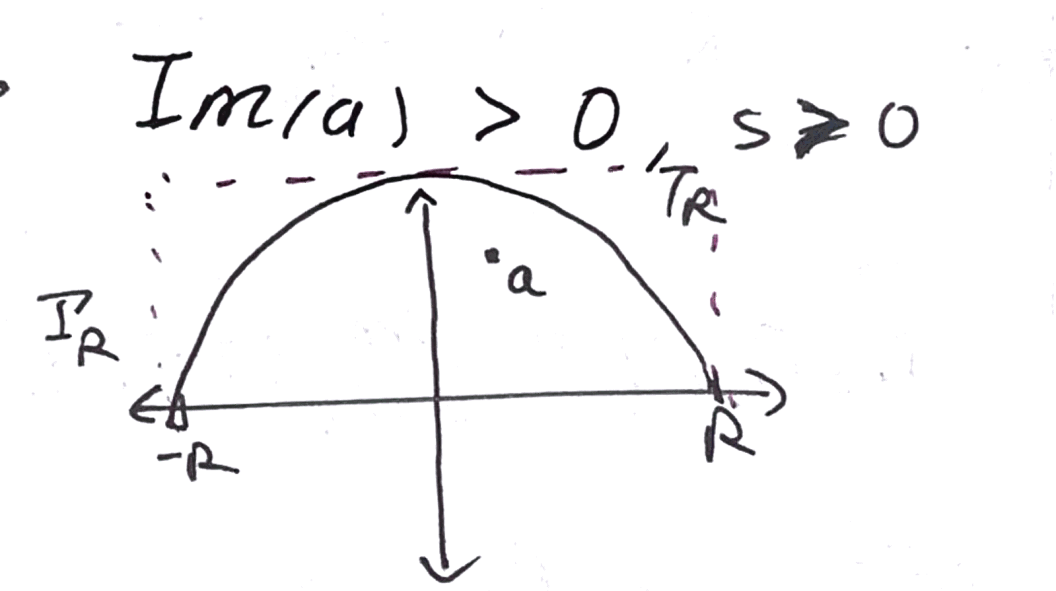
\includegraphics[width=.5\textwidth]{Figures/contour-3.png}}\]
where $R > |a|$, while we could use a rectangle, we will stick with the half-circle again. Then again Cauchys' Residue Theorem tells us that
\[\int_{\Gamma_R} f(z) dz = 2\pi i Res(f, a)\]
$a$ is a pole of order $1$ of $f$, so we have that
\[Res(f, a) = \lim_{z \to a} (z - a) \frac{e^{isz}}{z - a} = e^{isa}\]
However, we note that $f$ is actually \textbf{NOT INTEGRABLE}, so the following limit need not exist
\[\lim_{R \to \infty} \int_{-R}^R f(x) dx\]
Howebver, if $\int_{T_R} f(z) dz = 0$, then the limit would exist, and we would have
\[\lim_{R \to \infty} \int_{-R}^R f(x) dx = 2 \pi i e^{isa} = p.v \int_{-\infty}^\infty f(x) dx\]
However, we run into a problem with doing $ML$-esitmate on $\int_{T_R} f(z) dz = 0$, because it turns out it'd give us
\[|\int_{T_R} f(z) dz| \leq \frac{R}{R - |a|} \pi \]
, which does not converge to $0$ as $R \to \infty$.\\

Fortunately, we do have a workaround:
\begin{lemma}[Jordan's Lemma]
Let $C \in \Rbb$ be some fixed constant, then
\[\int_{T_R} |e^{iz}| |dz| \leq C\]
, where $|dz|$ is with respect to the Lebesgue Measure of the unit circle.
\end{lemma}

Now take $z = R e^{i \theta}$, then $dz = i R e^{i \theta} d \theta$, so we have that $|dz| = R |d \theta|$.

\begin{corollary}
If $s > 0$, then 
\[\int_{T_R} |e^{iz}| |dz| \leq C(s)\]
, where $C(s)$ is some constant dependent on $s$.
\end{corollary}

\begin{remark}
Jordan's Lemma for circles are generally hard to show, so most textbooks only prove it on a rectangle instead:
\[\fbox{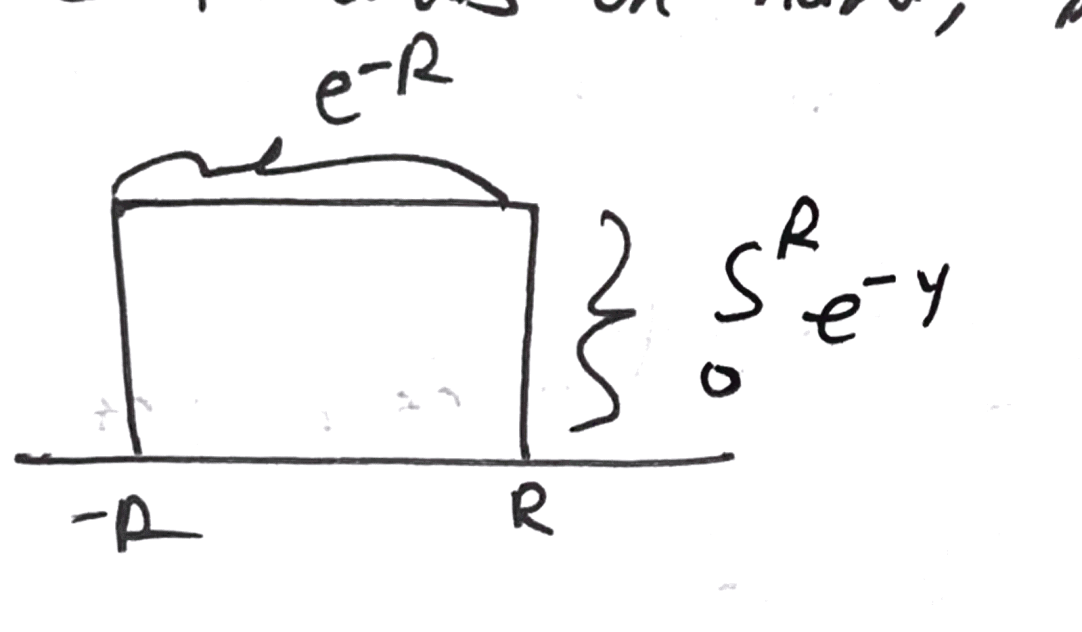
\includegraphics[width=.5\textwidth]{Figures/contour-4.png}}\]
\end{remark}

Now, using Jordan's Lemma, we have that
\begin{align*}
    |\int_{T_R} \frac{e^{isz}}{z - a} dz| &\leq \frac{1}{R - |a|} \cdot \int_{T_R} |e^{isz}| |dz|\\
    &\leq \frac{C(s)}{R - |a|}
\end{align*}
, so the limit goes to $0$ as $R \to \infty$.

\begin{question}
What about if $\Im(a) < 0$ and $s > 0$?
\end{question}

 In this case, we can either close the lower half or use a change of variables to get the same result.

\begin{question}
What about if $\Im(a) > 0$ but $s < 0$?
\end{question}

In this case, we will consider the contour
\[\fbox{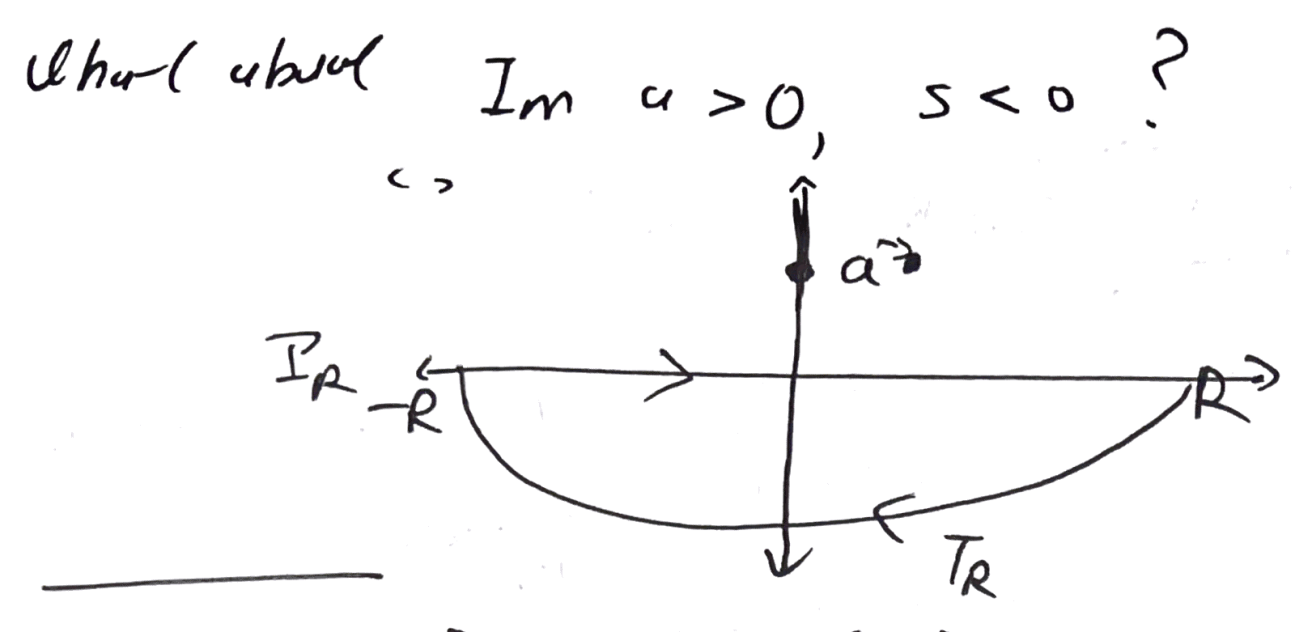
\includegraphics[width=.5\textwidth]{Figures/contour-5.png}}\]
There are no singularities inside the contour so
\[\int_{\Gamma_R} f(z) dz = 0\]
In addition, as $R \to \infty$, we also have that
\[\int_{T_R} f(z) dz = 0\]
Thus, the integral $I$ is just $0$.

\begin{question}
What if $a \in \Rbb \setminus \{0\}$ and $s > 0$?
\end{question}

In this case, consider the contour:
\[\fbox{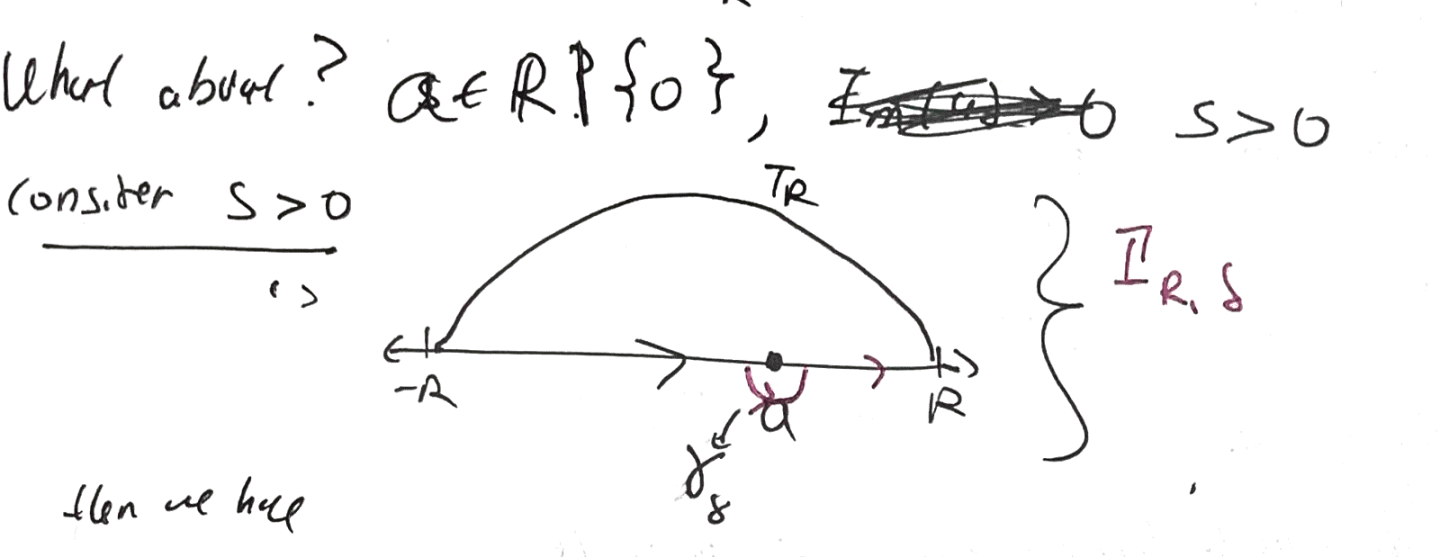
\includegraphics[width=.5\textwidth]{Figures/contour-6.png}}\]

In this, case we note that as we expand $R$ and shrink $\delta$, we have that
\[\int_{[-R, R] \setminus [a - \delta, a + \delta]} \mapsto p.v \int_{-\infty}^\infty f(z) dz\]

Cauchy's Residue Theorem tells us that
\[\int_{\Gamma_{R, \delta}} f(z) dz = 2 \pi i Res(f, a) = 2 \pi i e^{isa}\]

Jordan's Lemma tells us that
\[\lim_{R \to \infty} \int_{T_R} f(z) dz = 0 \]

Finally, taking $\delta \to 0$ gives that
\[\int_{\gamma_\delta} f(z) dz = \pi i e^{isa}\]

Thus, we have that
\[p.v \int_{-\infty}^\infty f(z) dz = 2 \pi i e^{isa} - \pi i e^{isa} = \pi i e^{isa}\]



\end{document}
